% REMEMBER: You must not plagiarise anything in your report. Be extremely careful.
\documentclass{l4proj}

    
%==============================================================================
% Put any additional packages here
% You can add any packages you want, as long as it does not alter
% the overall format (e.g. don't change the margins or the reference style).
%
\usepackage{pdfpages} % if you want to include a PDF for an ethics checklist, for example
%
%

\begin{document}

%==============================================================================
%% METADATA
\title{ENG5009 : Advanced Control 5\newline Laboratory Assignment\newline} % change this to your title
\author{Shivoh Chirayil Nandakumar (2456800C)}
\date{March 25 , 2020}

\maketitle

%==============================================================================

%==============================================================================


%==============================================================================
\tableofcontents

%==============================================================================
%% Notes on formatting
%==============================================================================
% The first page, abstract and table of contents are numbered using Roman numerals and are not
% included in the page count. 
%
% From now on pages are numbered
% using Arabic numerals. Therefore, immediately after the first call to \chapter we need the call
% \pagenumbering{arabic} and this should be called once only in the document. 
%
%
% The first Chapter should then be on page 1. 

% PAGE LIMITS
% You are allowed 40 pages for a 40 credit project and 30 pages for a 
% 20 credit report. 
% This includes everything numbered in Arabic numerals (excluding front matter) up
% to but *excluding the appendices and bibliography*.
%
% FORMATTING
% You must not alter text size (it is currently 10pt) or alter margins or spacing.
% Do not alter the bibliography style. 
%
%==================================================================================================================================
%
% IMPORTANT
% The chapter headings and structure here are **suggestions**. You don't have to follow this model if
% it doesn't fit your project. Every project should have an introduction and conclusion,
% however.  If in doubt, your supervisor can give you specific guidance; their view takes precedence over
% the structure suggested here.
%
%==================================================================================================================================
\chapter{Introduction}
The initial stage of the assignment is to familiarise and comprehend the working of various robust and intelligent control methods such as fuzzy logic and Neural Networks. Final stage of the assignment is to design a controller based on the above methods or any other suitable methods, that is able to guide a mobile robot to a particular point (within 0.05m radius of the point) while avoiding the obstacles. MATLAB was used for the modelling and simulation of the robot and controller.
% reset page numbering. Don't remove this!
\pagenumbering{arabic} 

% You can use \todo{} to mark text that needs to be fixed. Anything inside will appear as highlighted 
% text in the final copy, and you will also get warnings when you compile (so you don't
% forget to take them out!)

 
\chapter{Methodology}
The assignment can be divided into two parts 1) \textbf{Familiarisation of various type of Controllers and Robot simulation } 2)\textbf{Design and Implementation of the Suitable Controller}

\section{Familiarisation of various types of Controllers and Robot simulation}

\subsection{Robot Simulation}
Basic Manoeuvring of the robot was doable after understanding the codes inside functions. $runmodel.m$ ( used to run the robot simulation), $full\_mdl\_motors.m$ (Mathematical model of the Robot), drawbot.m (To Represent the robot in a figure), WallGeneration.m (to provide obstacle points to add into the $obs\_matrix ). Obs\_matrix$ is initialised with zeros. And as per the coordinates of the obstacles, the value of the $Obs\_matrix$ at that indices are changed to one. ObsSensor3.m (Which provide sensor outputs which can be utilised as inputs for our controllers).los\_auto 
\subsection{Fuzzy Controller}
A solid understanding of various aspects of Fuzzy Logic ToolBox such as Fuzzy Logic Designer, Membership function editor, Rule Editor, Rule Viewer, Surface viewer were obtained by creating Fuzzy systems for solving "the Basic Tipping Problem" and "the AC system" as per Laboratory worksheet 1. The results for the same are provided in the appendix. Moreover, A Fuzzy Controller was developed which allows the robot to avoid obstacles following the tutorial example \boldsymbol{comment}: The Fuzzy system was able to detect the obstacles and change the direction to avoid the obstacles. But, while moving at a higher speed, the fuzzy system was struggling to avoid the obstacles and sometimes went through the obstacles or took longer to react to a obstacle in front of it.. Further changes in the fuzzy rules made it avoid obstacles in a better way. \boldsymbol{Comment} : Various defuzzification methods such as Bisector, Centroid,Smallest of Maximum,Largest of Maximum and Mean of Maximum were tested to find the most suitable type of Defuzzification method for the given FIS variables. It was concluded from graphs of test results that, SOM and Bisector methods are the most suitable and MOM and LOM were the least suitable Defuzzification methods.Thus,applying Bisector method instead of the initial centroid method improves the efficiency of the Fuzzy controller for the robot.
\subsection{Neural Controller}
\newline
\begin{figure}[htb]
    \centering
    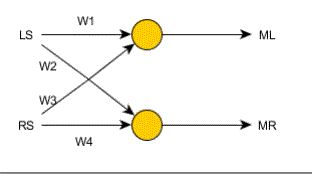
\includegraphics[width=0.5\linewidth]{images/Neural Pic.JPG}

    \caption{Simple Neural Network
    }

    % use the notation fig:name to cross reference a figure
    \label{fig:Rootlocus} 
\end{figure}
A neural network controller was created as a function in MATLAB according to figure of neural network given in the tutorial.The value to left neuron is obtained by summing the product of Left sensor and weight w1 with the product of right sensor and weight w3.Similarly,the value to right neuron is obtained by summing the product of Left sensor and weight w2 with the product of right sensor and weight w4. The value obtained in each neuron is compared with threshold values T1 and T2 for left and right neurons respectively. If the value is higher than the threshold, a positive voltage is given to the respective motor and else a negative voltage is given to that motor.  The neuron models were already trained and the trained weights and the thresholds were provided in the tutorial. The trained weights and the thresholds were given to the function along with the sensor outputs, to produce the desired output voltage for the Left and Right motors. Various trained weights and threshold were tested to find the best neural network for the obstacle avoidance. The results for the same are provided in the appendix.

\section{Design and Implementation of the Suitable Controller}
The Design and Implementation of the suitable controller is divided into to sections 1)\textbf{Movement of Robot to the desired points without Obstacles in the Arena} 2)\textbf{Movement of Robot to the desired points with Obstacles in the Arena}


\subsection{Without Obstacles}

The robot moves forward, backward or change direction according the the voltage we give to the right and left motors. And until now, the robot was allowed to move aimlessly through the arena and avoid any obstacles it encounters. So, in order to move the robot to a desired point it was given a sense of direction along which it should move, (desired Psi). Moreover a variable called "at\_waypoint" was created and the value of it is either 1 or 0 as whether the robot reached the desired point or not.\newline A function named los\_auto was created which takes in the present coordinates of the robot and the desired point, and gives the desired\_psi and at\_waypoint as the outputs. 
\newline Initially the code was tested by giving a single desired point. the los\_auto function was called inside the main loop of the run model. the desired\_psi obtained was set as value for xi(24).  at\_waypoint value was checked using an if statement and once the value is 1, the break command is given to end the loop.
\newline A matrix of desired points was created and a For loop was provided outside the main loop with number of iterations equal to number of desired points. Thus, when at\_waypoint value becomes 1, the main loop is stopped and outer loop starts the next iteration, in which the next desired point will be considered in the main loop. This continues until we reach the final destination.

\begin{figure}[htb]
    \centering
    \begin{subfigure}{0.45\textwidth}
        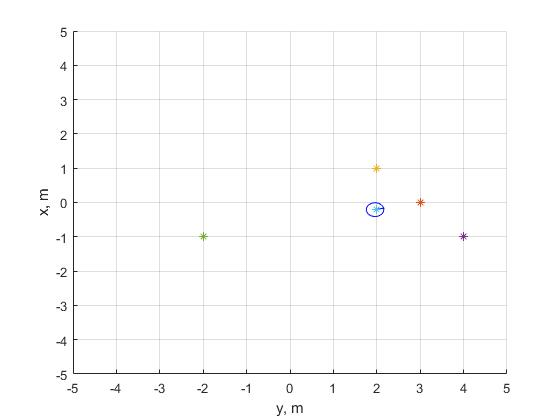
\includegraphics[width=\textwidth]{images/Plot task 1 1.jpg}
        \caption{Robot with desired Points (No Obstacles) }
        \label{fig:syn1}
    \end{subfigure}
     %add desired spacing between images, e. g. ~, \quad, \qquad, \hfill etc. 
      %(or a blank line to force the subfigure onto a new line)
    \begin{subfigure}{0.45\textwidth}
        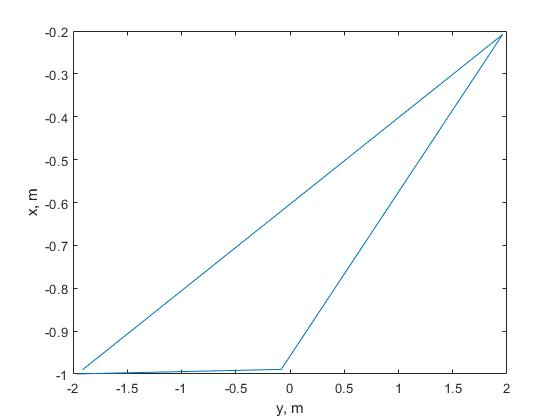
\includegraphics[width=\textwidth]{images/Plot task 1 2.jpg}
        \caption{Robot Trajectory}
        \label{fig:syn2}
    \end{subfigure} 
\end{figure}



\newpage
\subsection{With Obstacles}

A Fuzzy controller was designed to manoeuvre Robot through the obstacles following the suggestions given in the tutorial along with minor changes in rules and testing various defuzzification methods. Moreover, different Neural controllers were tested using the given trained weights and thresholds. Both controllers were giving similar results. The test results for all the cases are given in the Fuzzy controller and Neural Controller section of the appendix respectively. Fuzzy controller was finalised as it was more convenient for further fine tuning whenever necessary. 

\subsubsection{Design of Fuzzy Controller}

The design of fuzzy controller involves mainly 4 parts 1)Input FIS variables 2)Output FIS variables 3) Fuzzy Rules 4) Defuzzification Methods
\begin{figure}[htb]
    \centering
    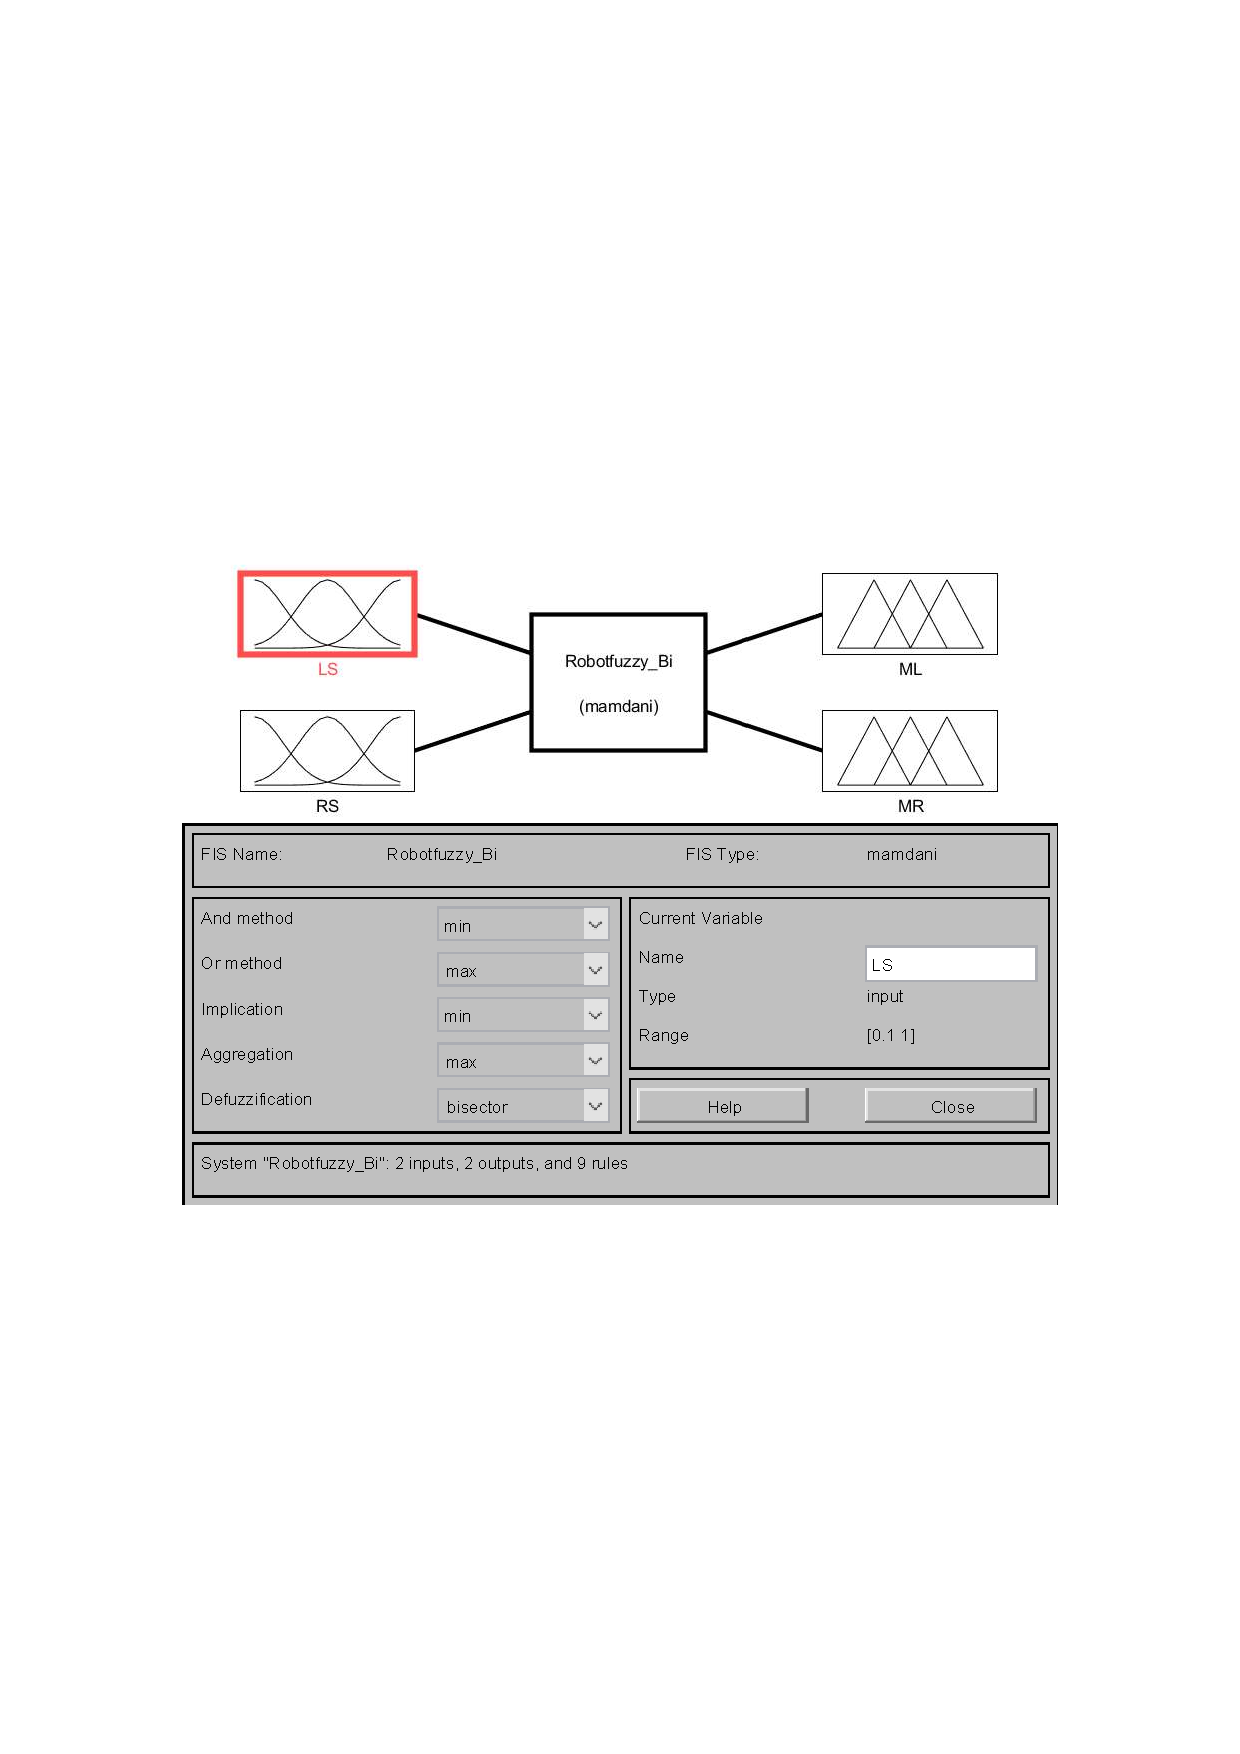
\includegraphics[width=0.5\linewidth]{images/fuzzy tool box.pdf}

    \caption{Fuzzy Controller
    }

    % use the notation fig:name to cross reference a figure
    \label{fig:Rootlocus} 
\end{figure}

Input FIS variables:  There are two input FIS (Fuzzy Inference System) variables, given as Left Sensor and Right Sensor. Each input FIS variable have 3 membership functions of trapezoid type named Too\_close, close and near.Trapezoid function was chosen due to the ease of applying the Too\_close, close and near to the obstacle  logic appropriately. The range of each Input FIS variable is [0,1].
\begin{figure}[htb]
    \centering
    \begin{subfigure}{0.45\textwidth}
        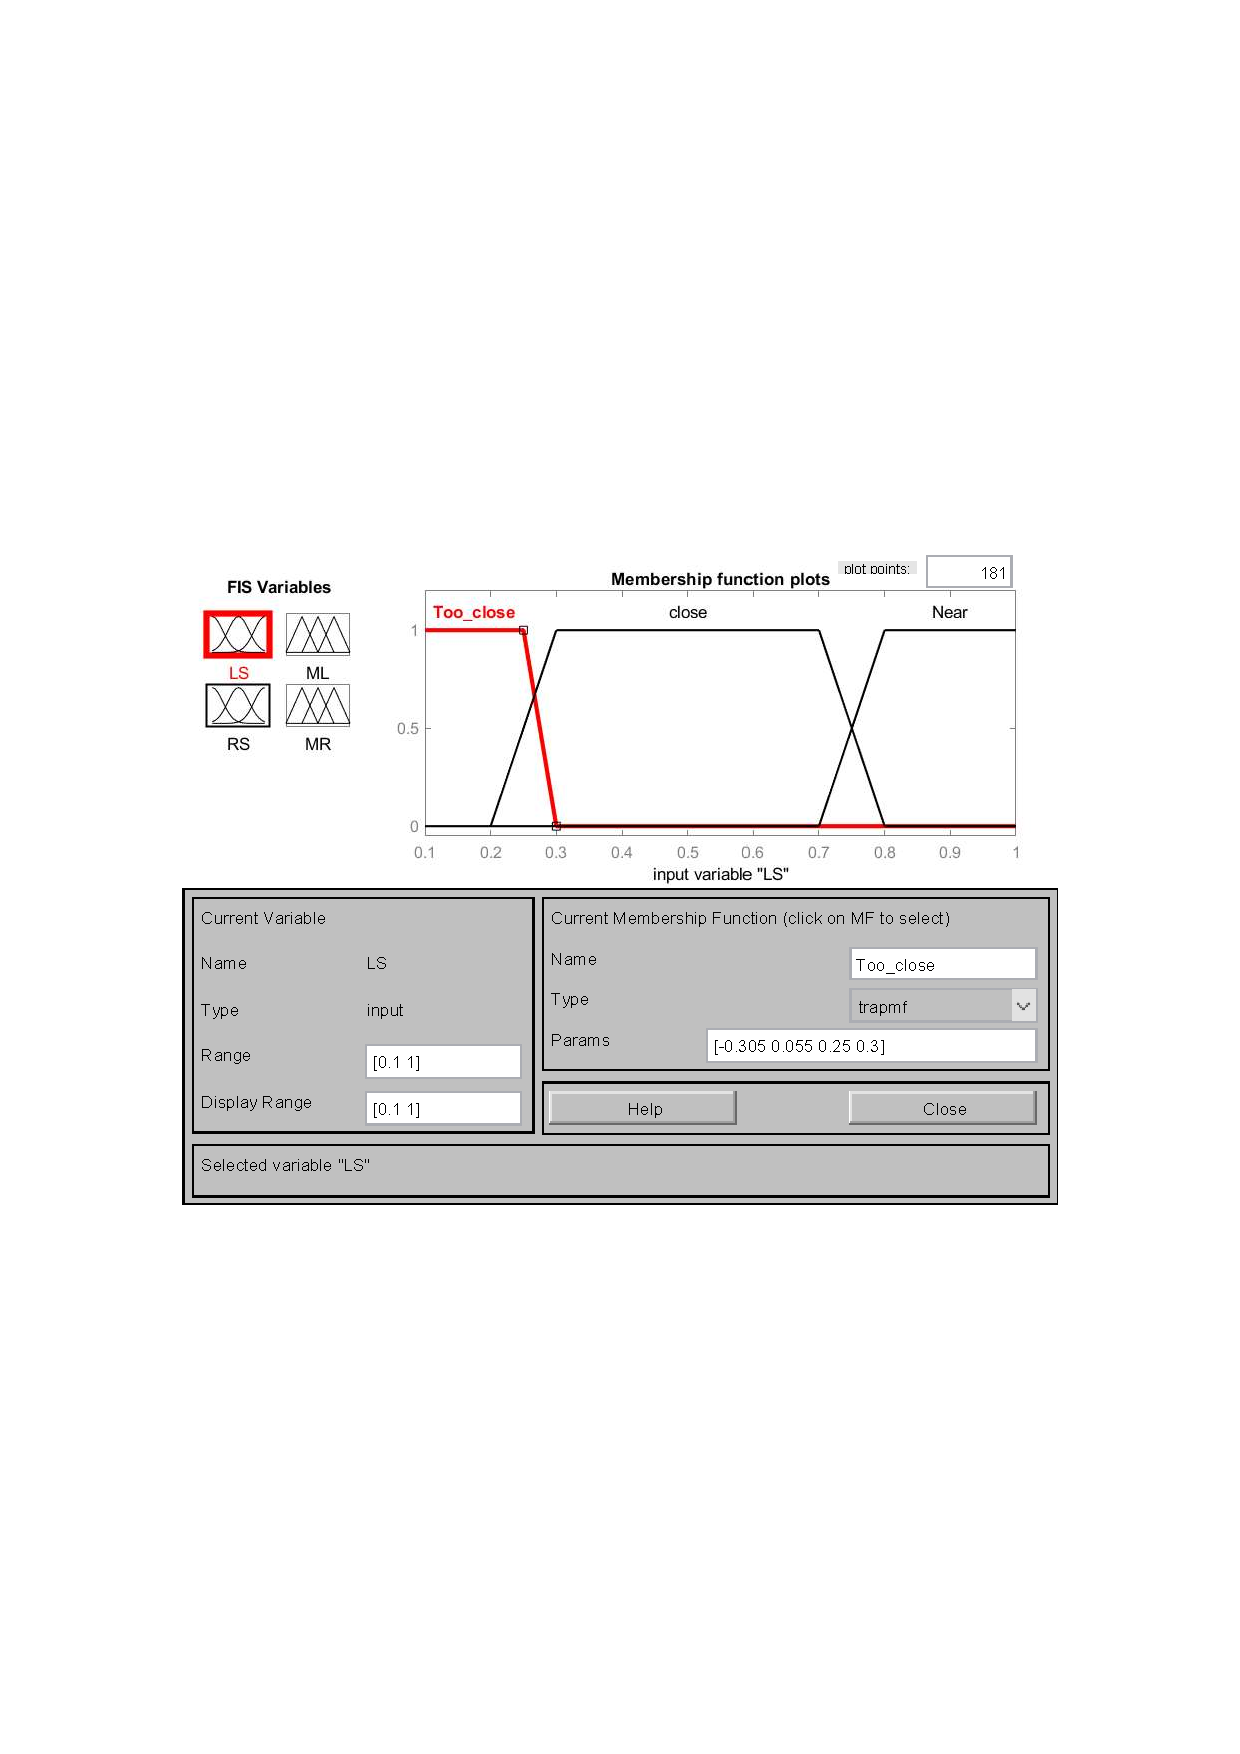
\includegraphics[width=\textwidth]{images/input functions.pdf}
        \caption{Input FIS variables and Membership Functions}
        \label{fig:syn1}
    \end{subfigure}
     %add desired spacing between images, e. g. ~, \quad, \qquad, \hfill etc. 
      %(or a blank line to force the subfigure onto a new line)
    \begin{subfigure}{0.45\textwidth}
        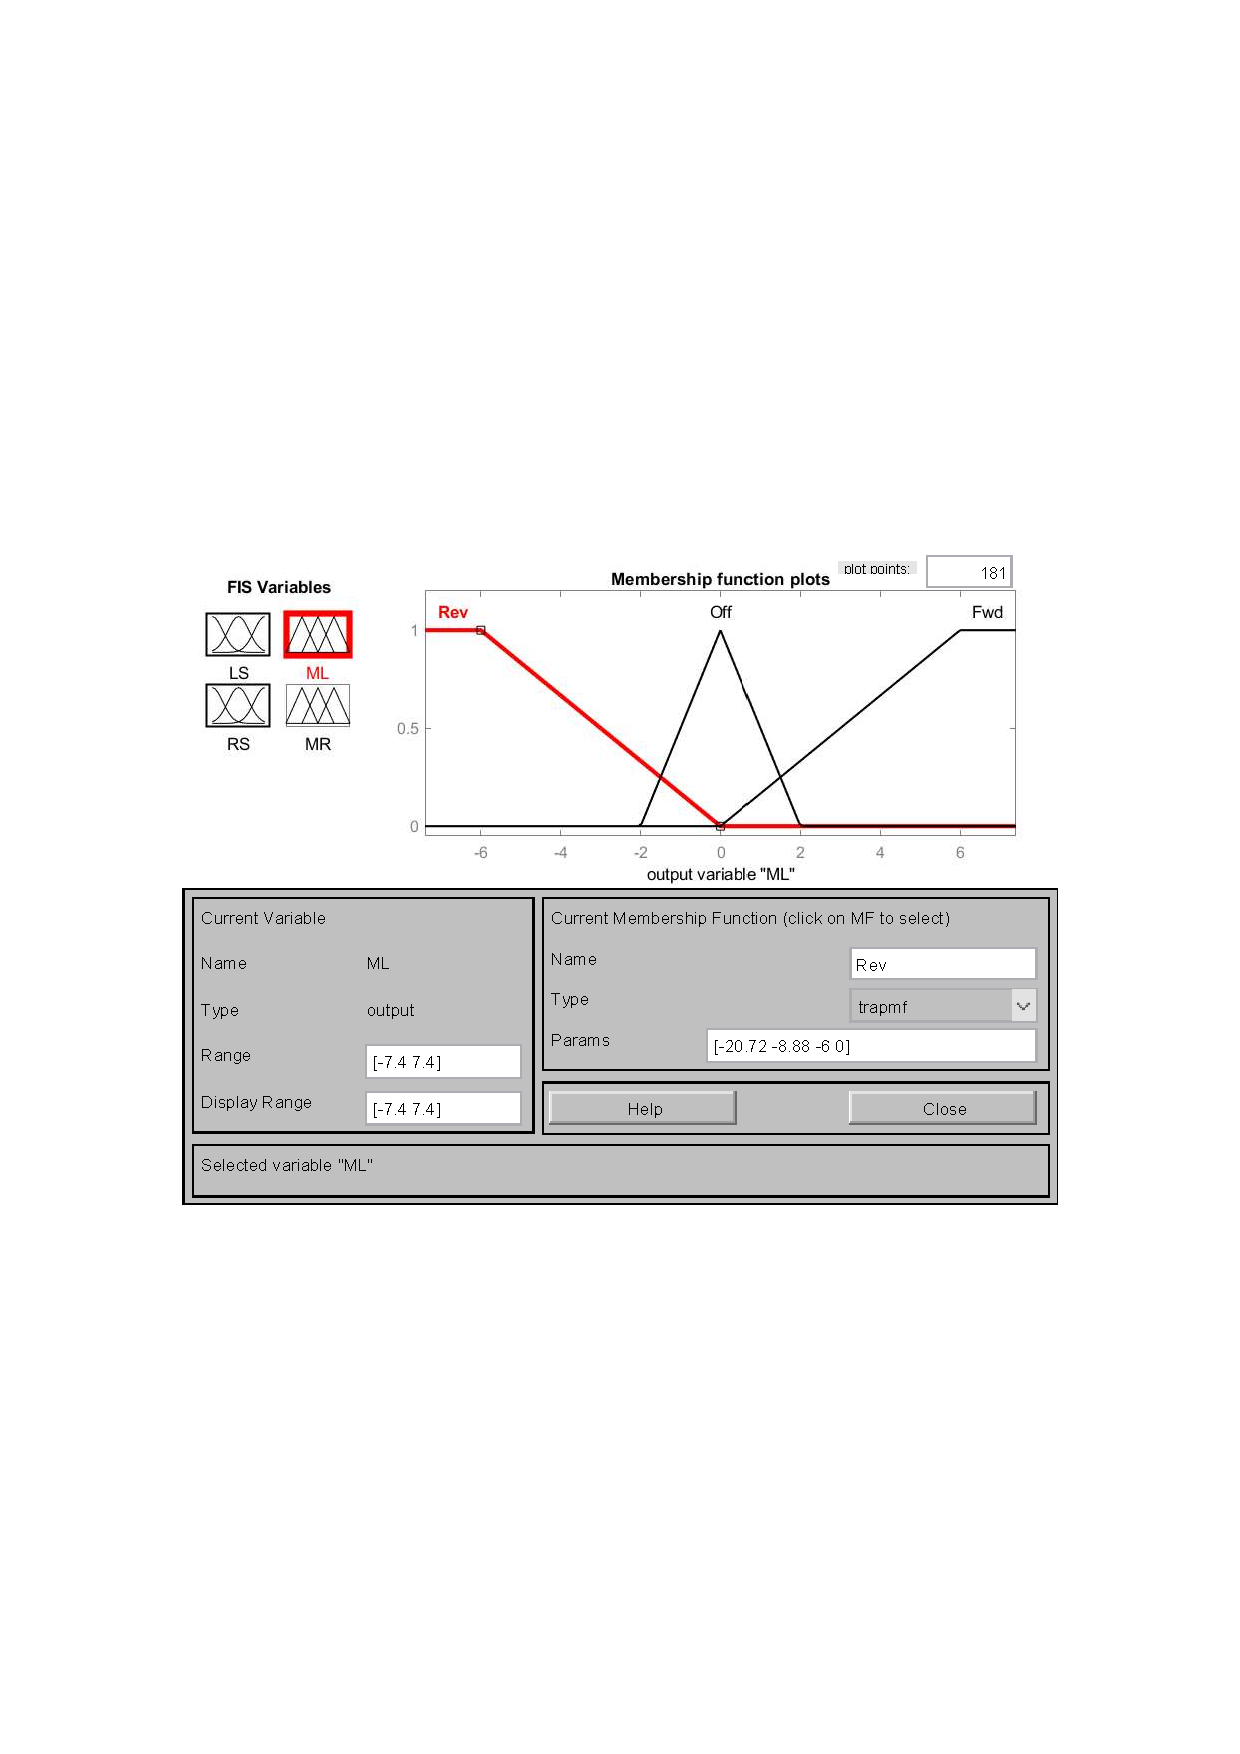
\includegraphics[width=\textwidth]{images/output fis.pdf}
        \caption{Output FIS variables and Membership Functions}
        \label{fig:syn2}
    \end{subfigure} 
\end{figure}
\newpage
Output FIS Variables: There are two output FIS (Fuzzy Inference System) variables, given as Left motor voltage and Right motor voltage. Each output FIS variable have 3 membership functions out of which 2 of them  are trapezoid type named Rev and Fwd, and one of them is of Triangular type named Off.The Trapezoid function was chosen due to the ease of applying the Reverse and Forward motion of the robot logically. a triangular function was chosen for 'Off' because we just need a single peak and a rapid decrease towards both sides.The range of each output FIS variable is [-7.4,7.4]. 7.4 was provided due to the fact that maximum value of voltage permissible to the motors is 7.4 Volts.

Fuzzy Rules: Considering the information provided in the tutorial, the rules for the fuzzy was developed. The rules were tested and further small changes were made to make the best movement possible to avoid the obstacles. No major alterations to the rules provided in the tutorials as almost all the test cases where successful using minor alterations. The initial and final fuzzy rules and the results for the same are provided in the appendix.
\newpage
\begin{figure}[htb]
    \centering
    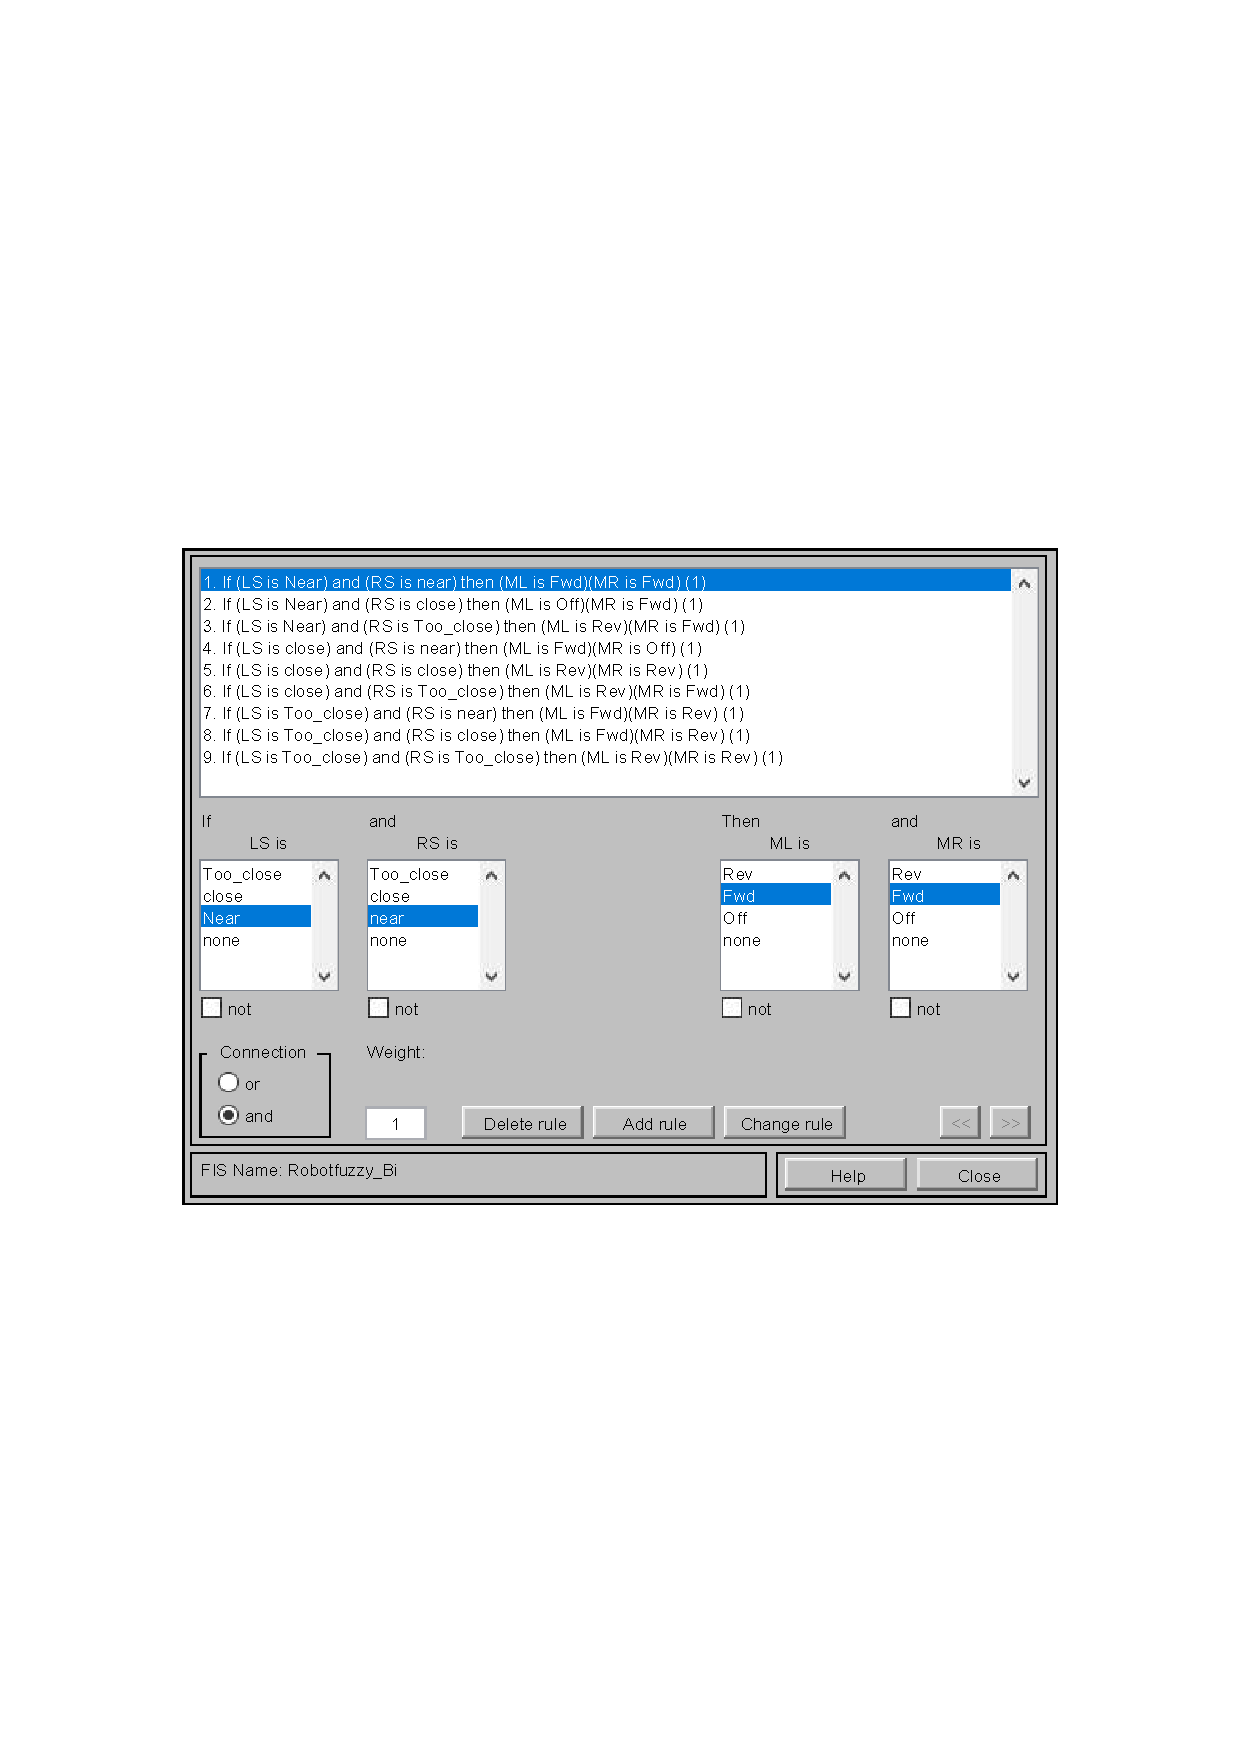
\includegraphics[width=0.5\linewidth]{images/rules.pdf}

    \caption{Rules for the Fuzzy System
    }

    % use the notation fig:name to cross reference a figure
    \label{fig:Rootlocus} 
\end{figure}

De-fuzzification Method: Various Defuzzification methods were tested and the variation obtained for each were thoroughly analysed. it was concluded that Mean of Maximum (MOM) and Largest of Maximum (LOM) were the least effective defuzzification methods for the given FIS Variables. Using MOM/LOM , the controller was not able to easily detect and change its manoeuvre when an obstacle was present. Centroid method was also not efficient, especially when the robot is moving at a good speed. it was not able to change its direction rapidly as soon as the obstacle was detected. Bisector and Smallest of Maximum were the best among the tested Defuzzification methods as the controller was able to change direction rapidly for all the test walls or the obstacles. Thus, Bisector defuzzification method was finalized for the Fuzzy Controller. The graph for each test are provided in the appendix.

\subsubsection{Programming for the simulation of Robot}

For both Fuzzy and Neural Controllers the Input is the output from the function ObsSensor3. The ObsSensor3 function takes in present position of the robot, position of the sensors, the psi angle and the obs\_matrix, and gives out values for left and right sensors depending on the distance from the obstacle in front of the robot.These values are given to the Fuzzy controller(or Neural) and the output voltage for the left and right motors are obtained from the controller.

 And as in the task one, a matrix of desired points were created and a For loop was provided outside the main loop with number of iterations equal to number of desired points. Thus, when at\_waypoint value becomes 1, the main loop is stopped and outer loop starts the next iteration, in which the next desired point will be considered in the main loop. This continues until we reach the final destination.

During the initial testing it was found that, the robot changes its direction as soon as it reach one of the desired point. And the desired points are arranged in such a way that no walls are near the trajectory of the robot. this means that, there was no movement which was obstructed by a wall in order to showcase the working of the Fuzzy controller. In other words, the robot might have reached the destination even if we haven't provided a fuzzy controller.So, a counter was created inside the main loop such that, the robot will move forward for a short while, even after reaching any of the  desired points(Except while reaching the destination). thus, the robot had a chance to encounter the walls and action of the fuzzy controller was clearly demonstrated.

The initial and final plots of the robot manoeuvre is provided in the appendix. 

\begin{figure}[htb]
    \centering
    \begin{subfigure}{0.45\textwidth}
        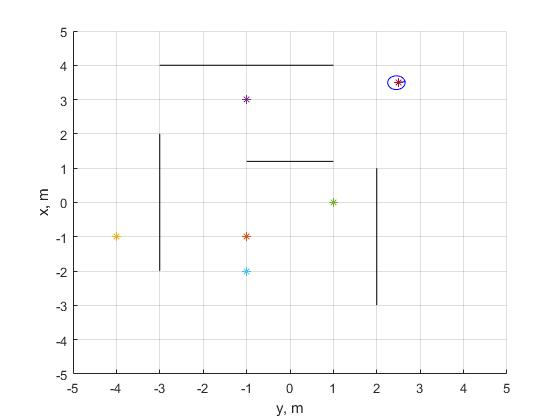
\includegraphics[width=\textwidth]{images/Robot.jpg}
        \caption{Final Map with Desired Points and Obstacles}
        \label{fig:syn1}
    \end{subfigure}
     %add desired spacing between images, e. g. ~, \quad, \qquad, \hfill etc. 
      %(or a blank line to force the subfigure onto a new line)
    \begin{subfigure}{0.45\textwidth}
        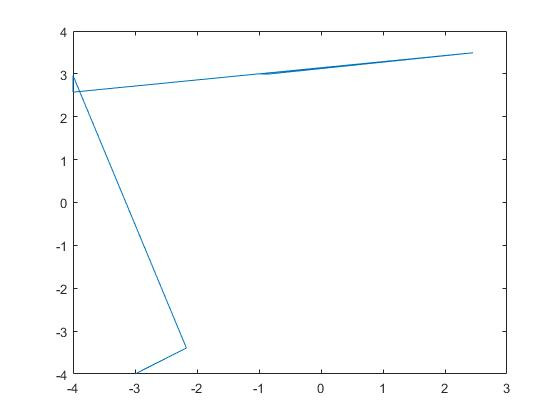
\includegraphics[width=\textwidth]{images/xy.jpg}
        \caption{Trajectory of Robot}
        \label{fig:syn2}
    \end{subfigure} 
\end{figure}

\section{Conclusion}
A Fuzzy Logic based Controller was designed , tested and Implemented to allow the mobile robot to move towards the desired points while avoiding the obstacles such as horizontal and vertical walls. After, various testing, Bisector method was used for the defuzzification in the given fuzzy controller, as it provided the best results as shown in the figures given in the appendix. The controller was able to successfully pass through all the required waypoints and reach the destination , while avoiding the Obstacles.  


\section{Improvements}
It was interesting to note that,extra waypoints had to be provided in order for the smooth movement of the robot to reach the final destination. \newline It is due to the fact that the neural controller we have is very basic  or the fuzzy system is only having basic rules and simple membership functions in the FIS variables. \newline Thus, It is possible that, with multiple hidden layers in the neural network and an efficient training of the neural controller by exposing it to more complex situations, the robot might be able to manoeuvre through the given grid in a much efficient manner.

\section{Appendix}

\subsection{Laboratory 1 Worksheet Answer Grid }
\begin{figure}[htb]
    \centering
    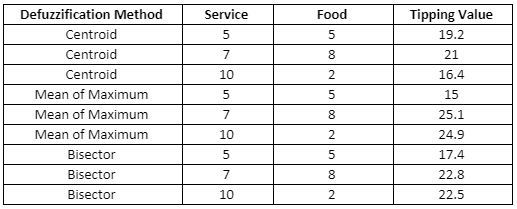
\includegraphics[width=0.5\linewidth]{images/Table1.JPG}    

    \caption{Introduction to Fuzzy Logic Toolbox 
    }

    % use the notation fig:name to cross reference a figure
    \label{fig:model1} 
\end{figure}

% Figures are important. Use them well.
\begin{figure}[htb]
    \centering
    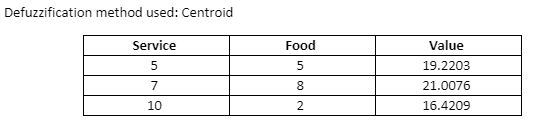
\includegraphics[width=0.5\linewidth]{images/Table2.JPG}    

    \caption{Integrating the Fuzzy system into the command line 
    }

    % use the notation fig:name to cross reference a figure
    \label{fig:model1} 
\end{figure}

\begin{figure}[htb]
    \centering
    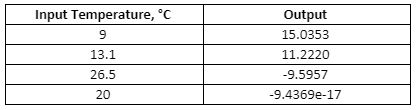
\includegraphics[width=0.5\linewidth]{images/table3.JPG}

    \caption{Further Fuzzy Logic Example 
    }

    % use the notation fig:name to cross reference a figure
    \label{fig:Model1sim1} 
\end{figure}
\begin{figure}[htb]
    \centering
    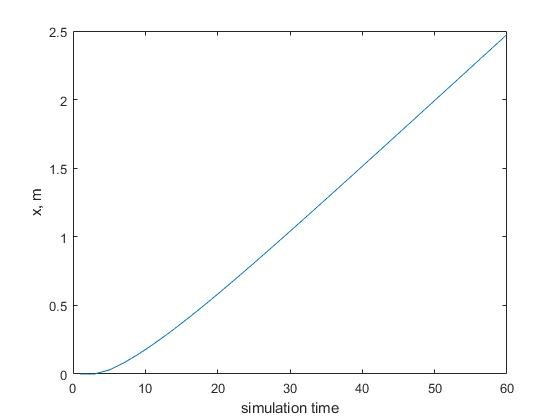
\includegraphics[width=0.5\linewidth]{images/Basic1.jpg}

    \caption{Basic Operation: Straight Line Motion
    }

    % use the notation fig:name to cross reference a figure
    \label{fig:Model1sim1} 
\end{figure}
\begin{figure}[htb]
    \centering
    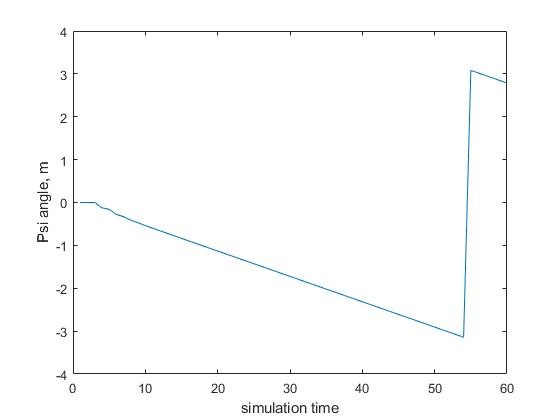
\includegraphics[width=0.5\linewidth]{images/Basic2.jpg}

    \caption{Basic Operation: Turn counterclockwise
    }
    \label{fig:Model1sim2} 
\end{figure}
\begin{figure}[htb]
    \centering
    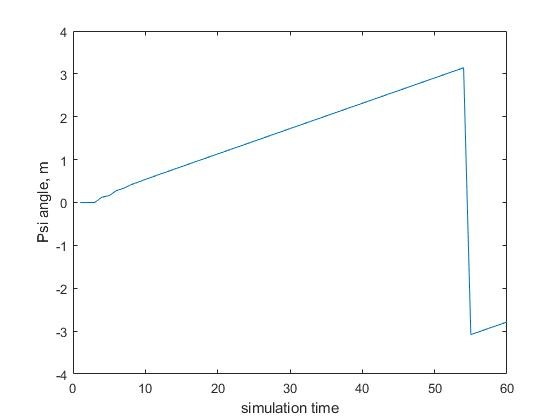
\includegraphics[width=0.5\linewidth]{images/Basic3.jpg}

    \caption{Basic Operation(Fuzzy): Turn Clockwise
    }
    \label{fig:Model1sim3} 
\end{figure}
    \begin{figure}[htb]
    \centering
    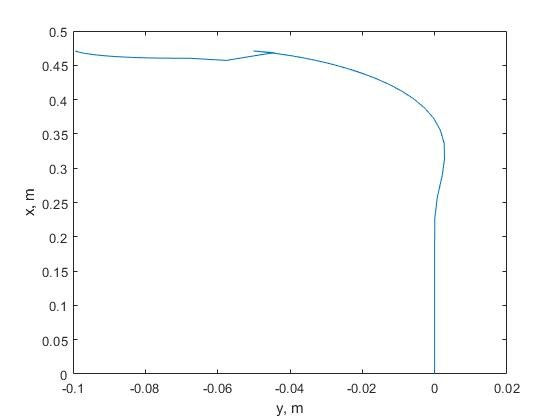
\includegraphics[width=0.5\linewidth]{images/Basic4.jpg}

    \caption{Basic Operation: Short forward, turn left, forward, turn right manoeuvre}
    \label{fig:Model1sim4} 
\end{figure}

\begin{figure}[htb]
    \centering
    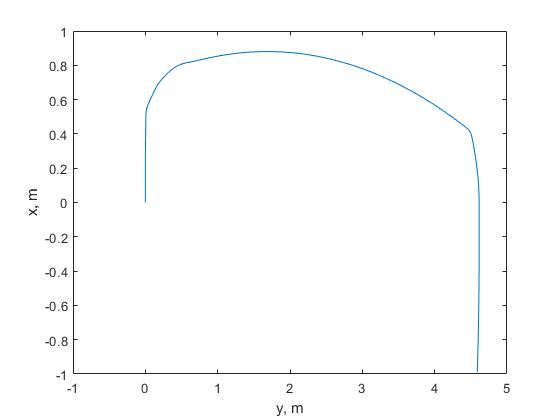
\includegraphics[width=0.5\linewidth]{images/initial xy plot.jpg}

    \caption{Basic Operation(Fuzzy): xy plot of robot with fuzzy controller as per tutorial}
    \label{fig:Model1sim4} 
\end{figure}
\begin{figure}[htb]
    \centering
    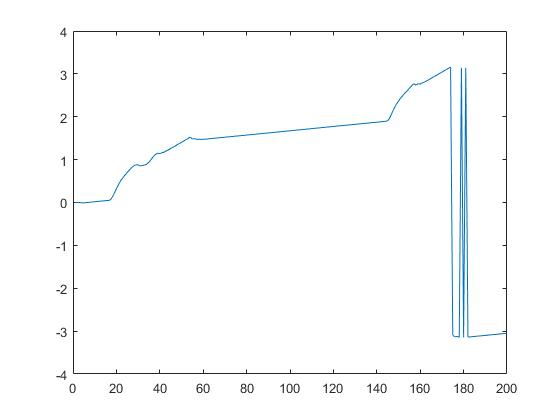
\includegraphics[width=0.5\linewidth]{images/Initial psi plot.jpg}

    \caption{Basic Operation(Fuzzy): psi angle variation of robot with fuzzy controller as per tutorial}
    \label{fig:Model1sim4} 
\end{figure}
\begin{figure}[htb]
    \centering
    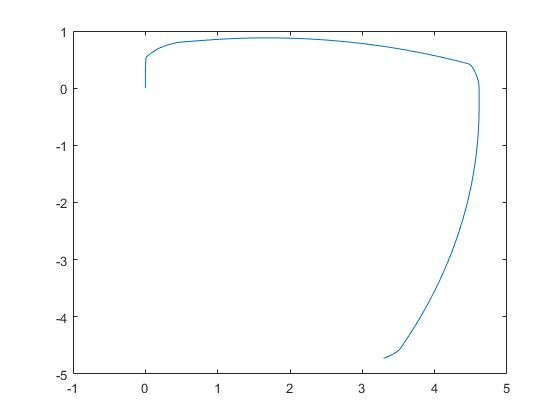
\includegraphics[width=0.5\linewidth]{images/cefig2.jpg}

    \caption{Basic Operation(Fuzzy): test 1 - Centroid Method}
    \label{fig:Model1sim4} 
\end{figure}
\begin{figure}[htb]
    \centering
    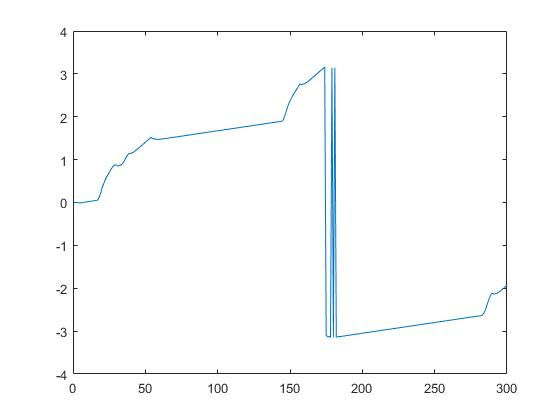
\includegraphics[width=0.5\linewidth]{images/cefig4.jpg}

    \caption{Basic Operation(Fuzzy): test 1 - Centroid Method, xy plot of robot}
    \label{fig:Model1sim4} 
\end{figure}
\begin{figure}[htb]
    \centering
    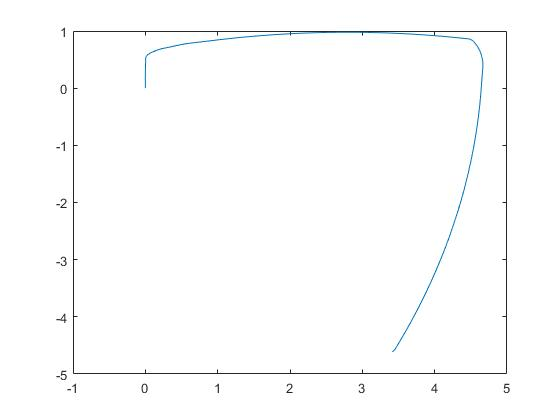
\includegraphics[width=0.5\linewidth]{images/bifig2.jpg}

    \caption{Basic Operation(Fuzzy): test 2 - Bisector Method}
    \label{fig:Model1sim4} 
\end{figure}
\begin{figure}[htb]
    \centering
    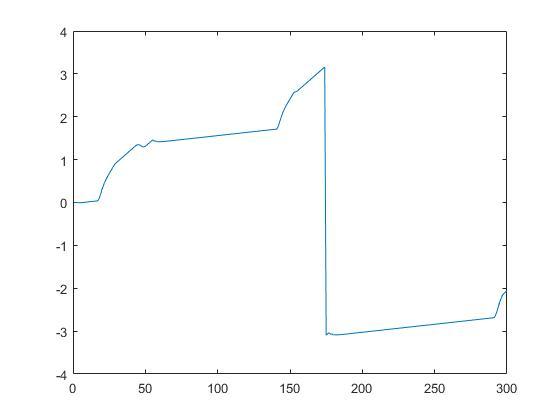
\includegraphics[width=0.5\linewidth]{images/bifig4.jpg}

    \caption{Basic Operation(Fuzzy): test 2 - Bisector Method, xy plot of robot}
    \label{fig:Model1sim4} 
\end{figure}
\begin{figure}[htb]
    \centering
    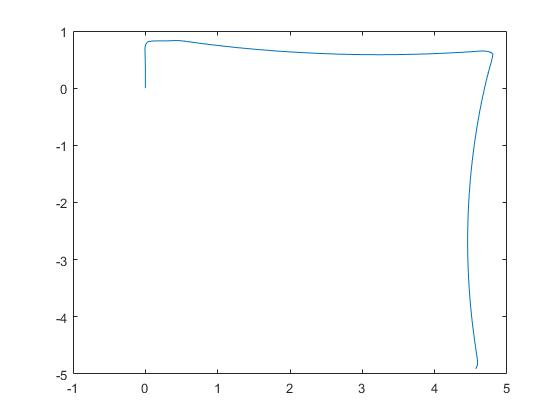
\includegraphics[width=0.5\linewidth]{images/Mofig2.jpg}

    \caption{Basic Operation(Fuzzy): test 3 - Mean Of Maximum (MOM) Method}
    \label{fig:Model1sim4} 
\end{figure}
\begin{figure}[htb]
    \centering
    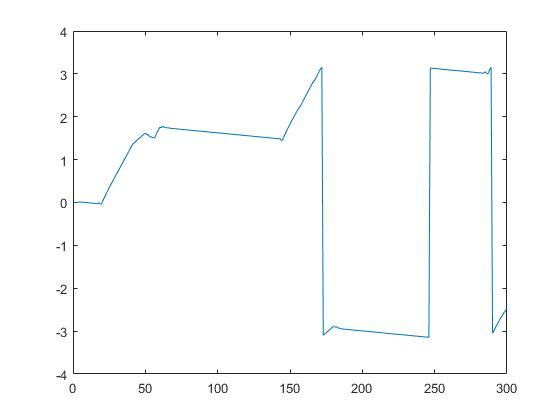
\includegraphics[width=0.5\linewidth]{images/Mofig4.jpg}

    \caption{Basic Operation(Fuzzy):Test 3 - Mean Of Maximum (MOM) Method xy plot of robot }
    \label{fig:Model1sim4} 
\end{figure}
\begin{figure}[htb]
    \centering
    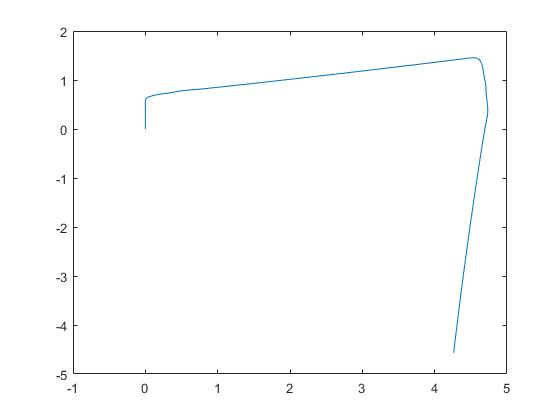
\includegraphics[width=0.5\linewidth]{images/sofig2.jpg}

    \caption{Basic Operation(Fuzzy): test 4 - Smallest Of Maximum (SOM) Method}
    \label{fig:Model1sim4} 
\end{figure}
\begin{figure}[htb]
    \centering
    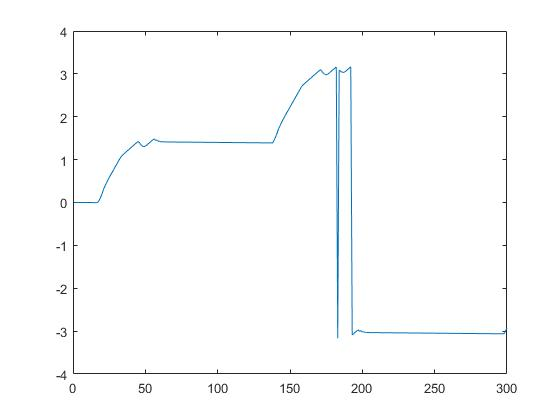
\includegraphics[width=0.5\linewidth]{images/sofig4.jpg}

    \caption{Basic Operation(Fuzzy): test 4 - Smallest Of Maximum (SOM) Method, xy plot of robot}
    \label{fig:Model1sim4} 
\end{figure}
\begin{figure}[htb]
    \centering
    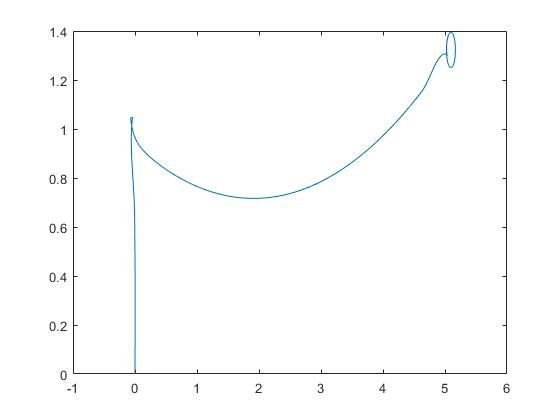
\includegraphics[width=0.5\linewidth]{images/lofig2.jpg}

    \caption{Basic Operation(Fuzzy): test 5 - Largest Of Maximum (LOM) Method}
    \label{fig:Model1sim4} 
\end{figure}
\begin{figure}[htb]
    \centering
    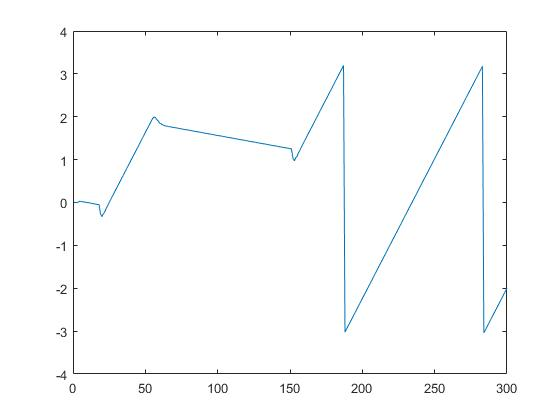
\includegraphics[width=0.5\linewidth]{images/lofig4.jpg}

    \caption{Basic Operation(Fuzzy): test 5 - Largest Of Maximum (LOM) Method, xy plot}
    \label{fig:Model1sim4} 
\end{figure}
\begin{figure}[htb]
    \centering
    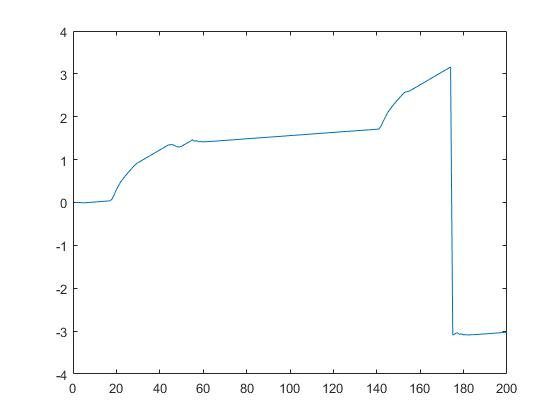
\includegraphics[width=0.5\linewidth]{images/final psi plot.jpg}

    \caption{Basic Operation(Fuzzy): psi angle variation of robot with improvised fuzzy controller}
    \label{fig:Model1sim4} 
\end{figure}
\begin{figure}[htb]
    \centering
    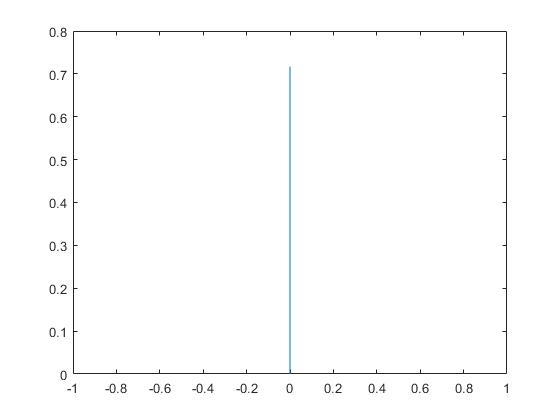
\includegraphics[width=0.5\linewidth]{images/Neuraltest1fig2.jpg}

    \caption{Basic Operation(Neural): xy plot of robot using neural controller (case-1)}
    \label{fig:Model1sim4} 
\end{figure}
\begin{figure}[htb]
    \centering
    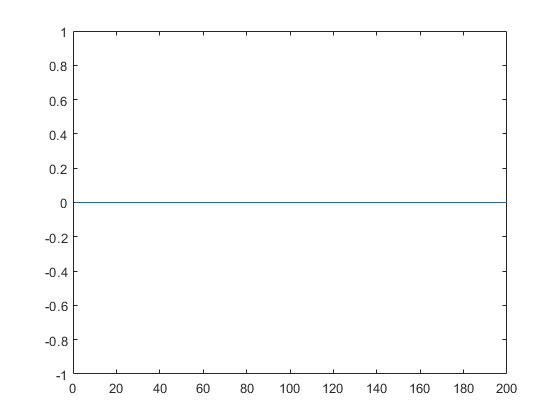
\includegraphics[width=0.5\linewidth]{images/Neuraltest1fig4.jpg}

    \caption{Basic Operation(Neural): psi angle variation of robot using neural controller (case-1)}
    \label{fig:Model1sim4} 
\end{figure}
\begin{figure}[htb]
    \centering
    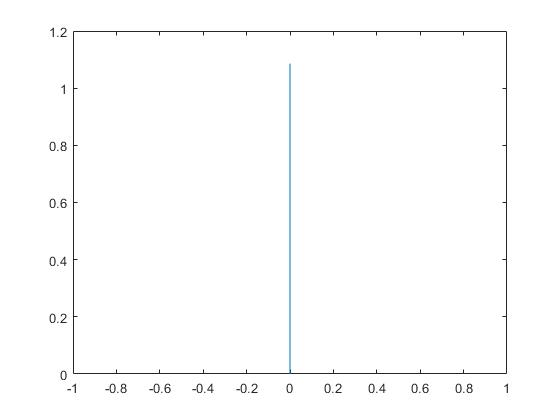
\includegraphics[width=0.5\linewidth]{images/Neuraltest2fig2.jpg}

    \caption{Basic Operation(Neural): xy plot of robot using neural controller (case-2)}
    \label{fig:Model1sim4} 
\end{figure}
\begin{figure}[htb]
    \centering
    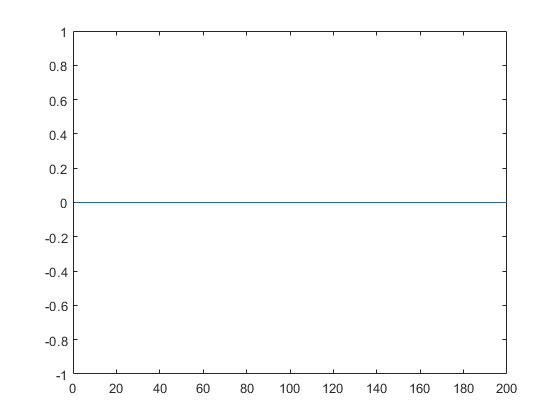
\includegraphics[width=0.5\linewidth]{images/Neuraltest2fig4.jpg}

    \caption{Basic Operation(Neural): psi angle variation of robot using neural controller (case-2)}
    \label{fig:Model1sim4} 
\end{figure}
\begin{figure}[htb]
    \centering
    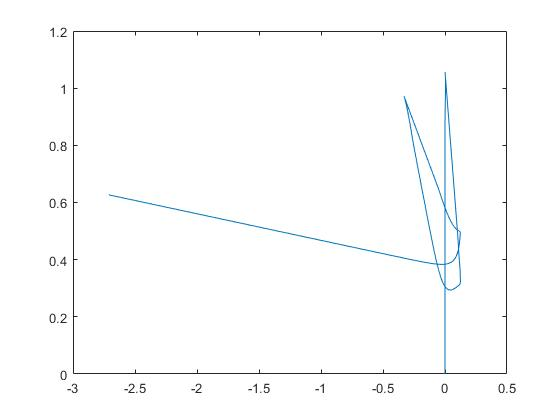
\includegraphics[width=0.5\linewidth]{images/Neuraltest3fig2.jpg}

    \caption{Basic Operation(Neural): xy plot of robot using neural controller (case-3)}
    \label{fig:Model1sim4} 
\end{figure}
\begin{figure}[htb]
    \centering
    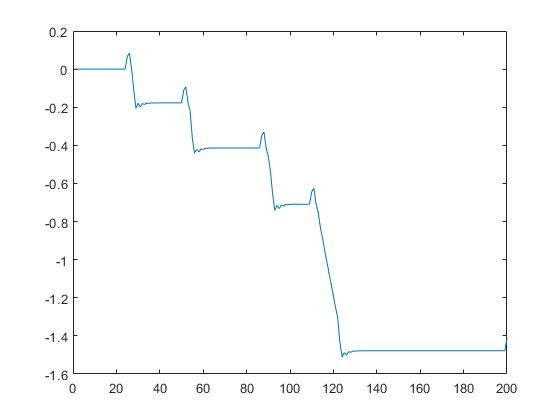
\includegraphics[width=0.5\linewidth]{images/Neuraltest3fig4.jpg}

    \caption{Basic Operation(Neural): psi angle variation of robot using neural controller (case-3)}
    \label{fig:Model1sim4} 
\end{figure}
\begin{figure}[htb]
    \centering
    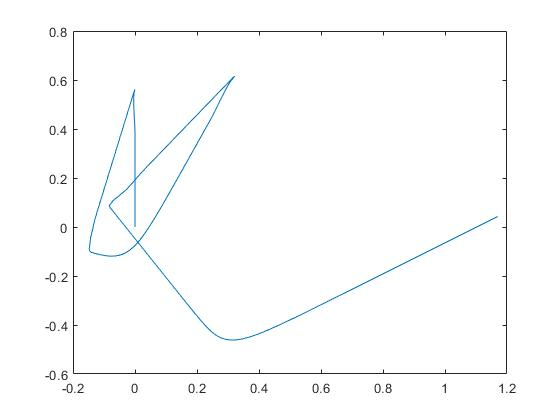
\includegraphics[width=0.5\linewidth]{images/Neuraltest4fig2.jpg}

    \caption{Basic Operation(Neural): xy plot of robot using neural controller (case-4)}
    \label{fig:Model1sim4} 
\end{figure}
\begin{figure}[htb]
    \centering
    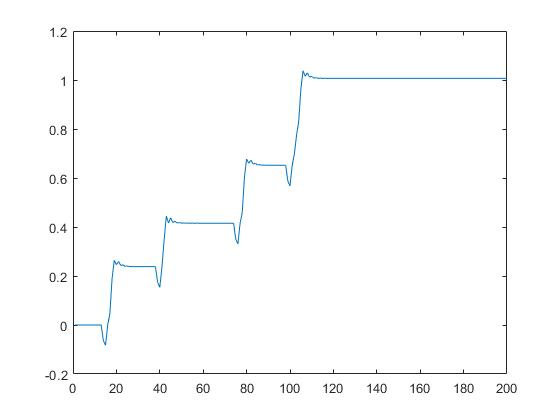
\includegraphics[width=0.5\linewidth]{images/Neuraltest4fig4.jpg}

    \caption{Basic Operation(Neural): psi angle variation of robot using neural controller (case-4)}
    \label{fig:Model1sim4} 
\end{figure}
\begin{figure}[htb]
    \centering
    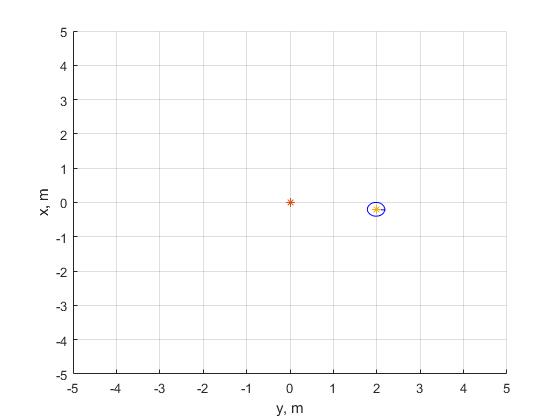
\includegraphics[width=0.5\linewidth]{images/Task1intialrobot.jpg}

    \caption{Task 1 (Testcase 1): robot with single desired point without any obstacles}
    \label{fig:Model1sim4} 
\end{figure}
\begin{figure}[htb]
    \centering
    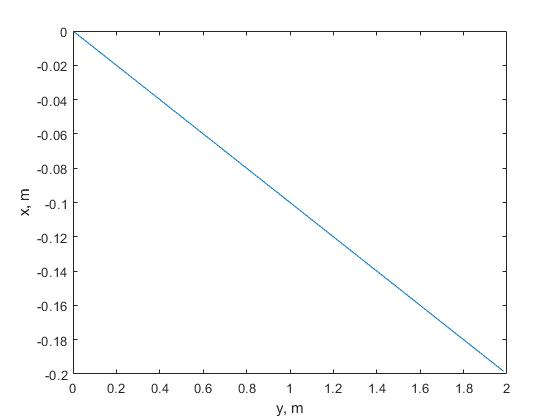
\includegraphics[width=0.5\linewidth]{images/Task1intialxyplot.jpg}

    \caption{Task 1 (Testcase 1): xy plot of robot with single desired point without any obstacles}
    \label{fig:Model1sim4} 
\end{figure}
\begin{figure}[htb]
    \centering
    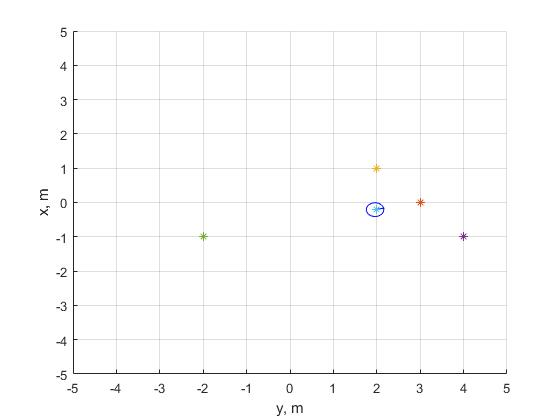
\includegraphics[width=0.5\linewidth]{images/Task1finalrobot.jpg}

    \caption{Task 1 (Final): robot with single desired point without any obstacles}
    \label{fig:Model1sim4} 
\end{figure}
\begin{figure}[htb]
    \centering
    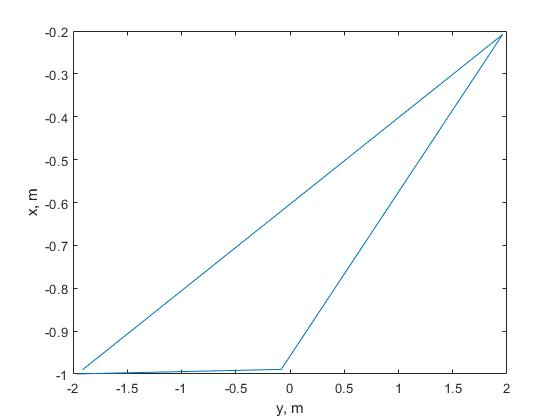
\includegraphics[width=0.5\linewidth]{images/Task1finalxyplot.jpg}

    \caption{Task 1 (Final): xy plot of robot with single desired point without any obstacles}
    \label{fig:Model1sim4} 
\end{figure}
\begin{figure}[htb]
    \centering
    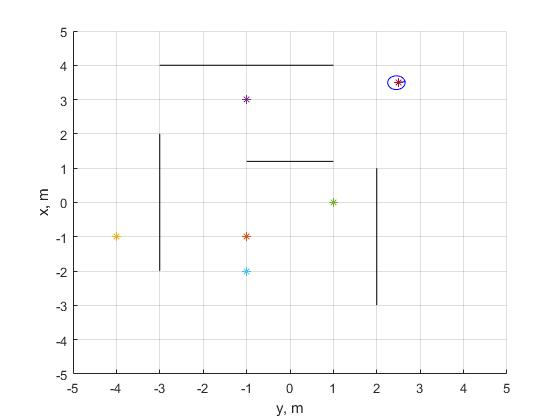
\includegraphics[width=0.5\linewidth]{images/Robot.jpg}

    \caption{Task 2 (testcase1): robot without extra waypoints}
    \label{fig:Model1sim4} 
\end{figure}
\begin{figure}[htb]
    \centering
    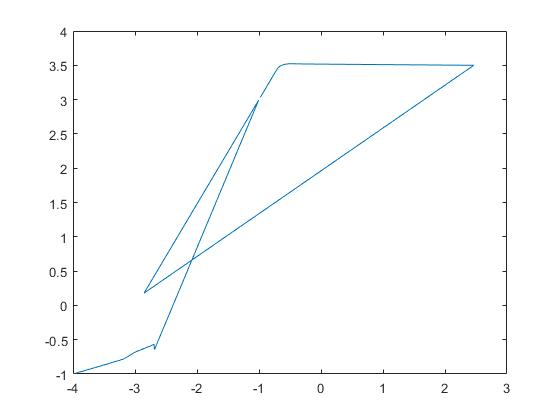
\includegraphics[width=0.5\linewidth]{images/task2test1xyplot.jpg}

    \caption{Task 2 (testcase1): xy plot of robot without extra waypoints (failed to avoid the walls)}
    \label{fig:Model1sim4} 
\end{figure}
\begin{figure}[htb]
    \centering
    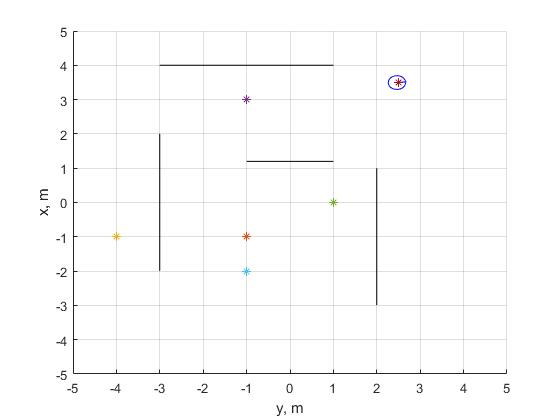
\includegraphics[width=0.5\linewidth]{images/task2test2robot.jpg}

    \caption{Task 2 (testcase2): robot with extra waypoints (Successfully avoided the walls)}
    \label{fig:Model1sim4} 
\end{figure}
\begin{figure}[htb]
    \centering
    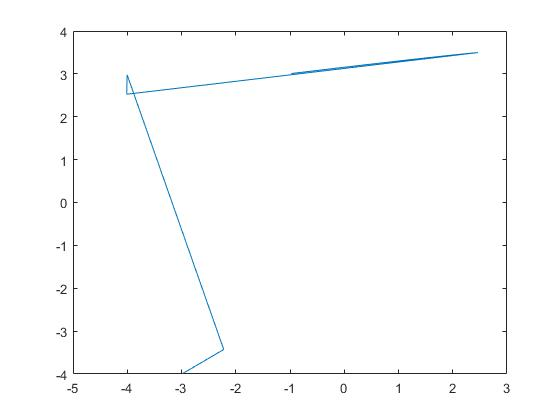
\includegraphics[width=0.5\linewidth]{images/task2test2xyplot.jpg}

    \caption{Task 2 (testcase2): xy plot of robot with extra waypoints}
    \label{fig:Model1sim4} 
\end{figure}
\begin{figure}[htb]
    \centering
    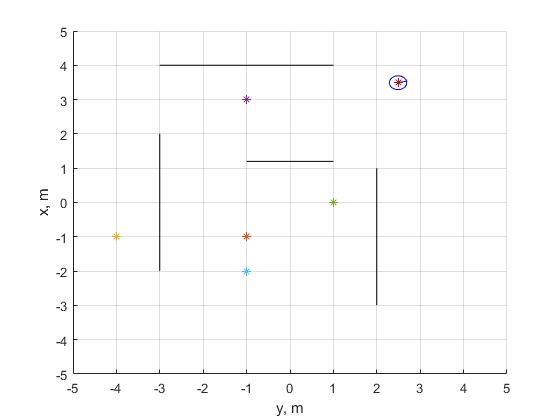
\includegraphics[width=0.5\linewidth]{images/task2test3robot.jpg}

    \caption{Task 2 (testcase3): With Counter: successfully avoids obstacles and reach the destination}
    \label{fig:Model1sim4} 
\end{figure}
\begin{figure}[htb]
    \centering
    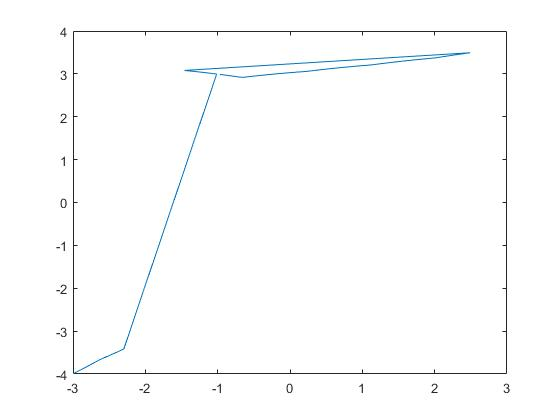
\includegraphics[width=0.5\linewidth]{images/task2test3xyplot.jpg}

    \caption{Task 2 (testcase3: xy plot of the robot (Final Case)}
    \label{fig:Model1sim4} 
\end{figure}

\newpage    
\newpage
\newpage

\newpage
\begin{lstlisting}[language=Matlab, float, caption={Code for short forward, turn left,forward,turn right manoeuvre
}, label=lst:callahan]
    if(outer_loop >(1.6/dT))
      Vl = 6;
      Vr = -6; 
    elseif(outer_loop > (1.56/dT))
      Vl = 6;
      Vr = 6;
    elseif(outer_loop > (0.32/dT))
      Vl = -6;
      Vr = 6;
    else
      Vl = 6;
      Vr = 6;
    end 
    \end{lstlisting}
   
\begin{lstlisting}[language=Matlab, float, caption={code for fuzzy controller (Basic Operation) }, label=lst:callahan]
    %----------------------------------------------%
    % Workspace Clear up
    close all;
    clear all;
    clc;
    %----------------------------------------------%

    %----------------------------------------------%
    % Setup Simulation
    Vl = 6;
    Vr = 6;
    sim_time = 10;
    dT = 0.05;
    xi = zeros(1,24); % intial state for x
    LeftS = 0;
    RightS = 0;
    Robotfuzzy = readfis('Robotfuzzy'); 
    %----------------------------------------------%

    %----------------------------------------------%
    % Create Environment
    max_x = 10;
    max_y = 10;

    Obs_Matrix = zeros(max_x/0.01,max_y/0.01);

    wall = WallGeneration1(-1, 1,1.2,1.2,'h');
    wall2 = WallGeneration1(-3, -3, -2, 2,'v');

    for x=1:length(wall)
    
    xpos = (wall(x,1)/0.01)+((max_x/2)/0.01);
    ypos = (wall(x,2)/0.01)+((max_y/2)/0.01);
    
    Obs_Matrix(ypos,xpos) = 1;
    end

    for x=1:length(wall2)
    
    xpos = (wall2(x,1)/0.01)+((max_x/2)/0.01);
    ypos = (wall2(x,2)/0.01)+((max_y/2)/0.01);
    
    Obs_Matrix(ypos,xpos) = 1;
    end
    %----------------------------------------------%

    %----------------------------------------------%
    for outer_loop = 1:(sim_time/dT)

    %----------------------------------------------%
    % Run Model
    sensorout = ObsSensor3(xi(19),xi(20),[0.2 0],xi(24),Obs_Matrix);
    motorpower = evalfis(Robotfuzzy,sensorout);
    V1 = motorpower(1);
    Vr = motorpower(2);
    Va = [Vl; Vl; Vr; Vr];
    [xdot, xi] = full_mdl_motors(Va,xi,0,0,0,0,dT);   
    xi = xi + (xdot*dT); % Euler intergration
    
    % Store varibles
    xdo(outer_loop,:) = xdot;
    xio(outer_loop,:) = xi;
    %----------------------------------------------%
  \end{lstlisting}    
 \begin{lstlisting}[language=Matlab, float, caption={
continuation from above page}, label=lst:callahan]   
    %----------------------------------------------%
    figure(1);
    clf; hold on; grid on; axis([-5,5,-5,5]);
    drawrobot(0.2,xi(20),xi(19),xi(24),'b');
    xlabel('y, m'); ylabel('x, m');
    plot(wall(:,1),wall(:,2),'k-');
    plot(wall2(:,1),wall2(:,2),'k-');
    pause(0.001);
    %----------------------------------------------%
    
    end
    %----------------------------------------------%

    %----------------------------------------------%
    %Plot Variables
    figure(2); plot(xio(:,20),xio(:,19));
    xlabel('y, m'); ylabel('x, m');
    figure(3); plot(xio(:,19));
    figure(4); plot(xio(:,24));
    %----------------------------------------------%



\end{lstlisting}
\begin{lstlisting}[language=Matlab, float, caption={Neural controller}, label=lst:callahan]
         function[Vl,Vr]=NeuralControl1(LeftS,RightS,weights,NeuralPara)
         %T1 and T2 are the respective threshold values for left and right neuron
         T1 = NeuralPara(1);
         T2 = NeuralPara(2);
        % w1,w2,w3,w4 represents the respective weights as per the diagram given in
        % Laboratory worksheet
        w1 = weights(1);
        w2 = weights(2);
        w3 = weights(3);
        w4 = weights(4);
    
        % value of left neuron
        Left_neural = w1*LeftS+w3*RightS;
    
        if Left_neural>T1
            Vl = 6;
        else
            Vl = - 6;
        end
    
        %value of right neuron
        Right_neural = w2*LeftS+w4*RightS;
    
        if Right_neural>T2
            Vr = 6;
        else
            Vr =- 6;
        end
        end
\end{lstlisting}
\begin{lstlisting}[language=Matlab, float, caption={Code implementing Neural controller
}, label=lst:callahan]
    %----------------------------------------------%
    % Workspace Clear up
    close all;
    clear all;
    clc;
    %----------------------------------------------%
    
    %----------------------------------------------%
    % Setup Simulation
    Vl = 6;
    Vr = 6;
    sim_time = 10;
    dT = 0.05;
    xi = zeros(1,24); % intial state for x
    LeftS = 0;
    RightS = 0;
    %Neural settings
    %test 1
    % NeuralPara = [0.3,0.3];
    % weights = [0.05,0.35,0.35,0.05];
    %test 2
    % NeuralPara = [0.3,0.3];
    % weights = [0.15,0.6,0.6,0.15];
    %test 3
    % NeuralPara = [0.15,0.15];
    % weights = [-0.2,0.6,0.5,-0.2];
    % %test 4
    NeuralPara = [5,5];
    weights = [1.39,3.83,4.79,1.59];
    
    %----------------------------------------------%
    
    %----------------------------------------------%
    % Create Environment
    max_x = 10;
    max_y = 10;
    
    Obs_Matrix = zeros(max_x/0.01,max_y/0.01);
    
    wall = WallGeneration1(-1, 1,1.2,1.2,'h');
    wall2 = WallGeneration1(-3, -3, -2, 2,'v');
    
    for x=1:length(wall)
        
        xpos = (wall(x,1)/0.01)+((max_x/2)/0.01);
        ypos = (wall(x,2)/0.01)+((max_y/2)/0.01);
        
        Obs_Matrix(ypos,xpos) = 1;
    end
    
    for x=1:length(wall2)
        
        xpos = (wall2(x,1)/0.01)+((max_x/2)/0.01);
        ypos = (wall2(x,2)/0.01)+((max_y/2)/0.01);
        
        Obs_Matrix(ypos,xpos) = 1;
    end
    %----------------------------------------------%
    
    %----------------------------------------------%
    
    for outer_loop = 1:(sim_time/dT)
\end{lstlisting}

\begin{lstlisting}[language=Matlab, float, caption={Code implementing Neural controller}, label=lst:callahan]
    %----------------------------------------------%
    % Run Model
    sensorout = ObsSensor3(xi(19),xi(20),[0.2 0],xi(24),Obs_Matrix);
    [Vl, Vr] = NeuralControl1(sensorout(1),sensorout(2),weights,NeuralPara);
    Va = [Vl; Vl; Vr; Vr];
    [xdot, xi] = full_mdl_motors(Va,xi,0,0,0,0,dT);   
    xi = xi + (xdot*dT); % Euler intergration
    
    % Store varibles
    xdo(outer_loop,:) = xdot;
    xio(outer_loop,:) = xi;
    %----------------------------------------------%
    
    %----------------------------------------------%
    figure(1);
    clf; hold on; grid on; axis([-5,5,-5,5]);
    drawrobot(0.2,xi(20),xi(19),xi(24),'b');
    xlabel('y, m'); ylabel('x, m');
    plot(wall(:,1),wall(:,2),'k-');
    plot(wall2(:,1),wall2(:,2),'k-');
    pause(0.001);
    %----------------------------------------------%
    
    end
    %----------------------------------------------%
    
    %----------------------------------------------%
    %Plot Variables
    figure(2); plot(xio(:,20),xio(:,19));
    figure(3); plot(xio(:,19));
    figure(4); plot(xio(:,24));
    %----------------------------------------------%

    \end{lstlisting}
    
\begin{lstlisting}[language=Matlab, float, caption={Task 1 ,Single desired Point (Test 1)}, label=lst:callahan]
     % Workspace Clear up
    close all;
    clear all;
    clc;
    %----------------------------------------------%
    
    %----------------------------------------------%
    % Setup Simulation
    Vl = 6;
    Vr = 6;
    sim_time = 15;
    xlabel('y, m'); 
    ylabel('x, m');
    dT = 0.05;
    xi = zeros(1,24); % intial state for x
    LeftS = 0;
    RightS = 0;
    desired_pt = [-0.2,2];
    %----------------------------------------------%
    
    %----------------------------------------------%
    % Create Environment
    max_x = 10;
    max_y = 10;
    
    
    
    %----------------------------------------------%
    for outer_loop = 1:(sim_time/dT)

    %----------------------------------------------%
    % Run Model
    
    [at_waypoint,xi(24)] = los_auto(xi(19),xi(20),desired_pt);
    
    
    Va = [Vl; Vl; Vr; Vr];
    [xdot, xi] = full_mdl_motors(Va,xi,0,0,0,0,dT);   
    xi = xi + (xdot*dT); % Euler intergration
    
    % Store varibles
    xdo(outer_loop,:) = xdot;
    xio(outer_loop,:) = xi;
    %----------------------------------------------%
        \end{lstlisting}
 \begin{lstlisting}[language=Matlab, float, caption={Task 1 ,Single desired Point (Test 1)}, label=lst:callahan]   
    %----------------------------------------------%
    figure(1);
    clf; hold on; grid on; axis([-5,5,-5,5]);
    drawrobot(0.2,xi(20),xi(19),xi(24),'b');
    xlabel('y, m'); ylabel('x, m');
    plot(0,0,'*');
    plot(desired_pt(2),desired_pt(1),'*');
    
    pause(0.001);
    %----------------------------------------------%
    if at_waypoint ==1
        break
    end

    end
    %----------------------------------------------%
    
    %----------------------------------------------%
    %Plot Variables
    figure(2); plot(xio(:,20),xio(:,19));
    xlabel('y, m'); ylabel('x, m');
    figure(3); plot(xio(:,19));
    figure(4); plot(xio(:,24));
    %----------------------------------------------%    
    \end{lstlisting}
\begin{lstlisting}[language=Matlab, float, caption={Task 1 , Final  Code}, label=lst:callahan]       
    %----------------------------------------------%
    % Workspace Clear up
    close all;
    clear all;
    clc;
    %----------------------------------------------%
    
    %----------------------------------------------%
    % Setup Simulation
    Vl = 6;
    Vr = 6;
    sim_time = 15;
    xlabel('y, m'); 
    ylabel('x, m');
    dT = 0.05;
    xi = zeros(1,24); % intial state for x
    LeftS = 0;
    RightS = 0;
    
    %----------------------------------------------%
    
    %----------------------------------------------%
    % Create Environment
    max_x = 10;
    max_y = 10;
    
    
    %----------------------------------------------%
    desired_pt = [0,3;1,2;-1,4;-1,-2;-0.2,2];
    %----------------------------------------------%
    for i = 1:5
    for outer_loop = 1:(sim_time/dT)

    %----------------------------------------------%
    % Run Model
    
    [at_waypoint,xi(24)] = los_auto(xi(19),xi(20),desired_pt(i,:));
    
    
    Va = [Vl; Vl; Vr; Vr];
    [xdot, xi] = full_mdl_motors(Va,xi,0,0,0,0,dT);   
    xi = xi + (xdot*dT); % Euler intergration
    
    % Store varibles
    xdo(outer_loop,:) = xdot;
    xio(outer_loop,:) = xi;
    %----------------------------------------------%
 \end{lstlisting}
\begin{lstlisting}[language=Matlab, float, caption={Task 1 , Final code}, label=lst:callahan]       
    %----------------------------------------------%
    figure(1);
    clf; hold on; grid on; axis([-5,5,-5,5]);
    drawrobot(0.2,xi(20),xi(19),xi(24),'b');
    xlabel('y, m'); ylabel('x, m');
    plot(desired_pt(1,2),desired_pt(1,1),'*');
    plot(desired_pt(2,2),desired_pt(2,1),'*');
    plot(desired_pt(3,2),desired_pt(3,1),'*');
    plot(desired_pt(4,2),desired_pt(4,1),'*');
    plot(desired_pt(5,2),desired_pt(5,1),'*');
    pause(0.001);
    %----------------------------------------------%
    if at_waypoint ==1
        break
    end

    end
    end
    %----------------------------------------------%
    
    %----------------------------------------------%
    %Plot Variables
    figure(2); plot(xio(:,20),xio(:,19));
    xlabel('y, m'); ylabel('x, m');
    figure(3); plot(xio(:,19));
    figure(4); plot(xio(:,24));
    %----------------------------------------------%
 \end{lstlisting}
 
\begin{lstlisting}[language=Matlab, float, caption={Task 2 ,Without additional waypoints (Test 1)}, label=lst:callahan]    
     %----------------------------------------------%
    % Workspace Clear up
    close all;
    clear all;
    clc;
    %----------------------------------------------%
    
    %----------------------------------------------%
    % Setup Simulation
    Vl = 6;
    Vr = 6;
    sim_time = 12;
    dT = 0.05;
    xi = zeros(1,24); % intial state for x
    LeftS = 0;
    RightS = 0;
    initialposi = [-2,-1];
    xi(19)= initialposi(1);
    xi(20)= initialposi(2);
    %desired_pt =[-1, -1 ;0, 1 ;-1,1;-4,-3;-1 ,-4 ;3,-4; 3 ,-1 ;3.5,2.5];
    desired_pt =[-1, -1 ;0, 1 ;-1 ,-4; 3 ,-1 ;3.5,2.5];
    
    Robotfuzzy = readfis('Robotfuzzy_bi');
    %----------------------------------------------%
    
    %----------------------------------------------%
    % Create Environment
    max_x = 10;
    max_y = 10;
    
    Obs_Matrix = zeros(max_x/0.01,max_y/0.01);
    
    wall = WallGeneration1(-1, 1,1.2,1.2,'h');
    wall2 = WallGeneration1(-3, -3, -2, 2,'v');
    wall3 = WallGeneration1(-3, 1,4,4,'h');
    wall4 = WallGeneration1(2, 2, -3, 1,'v');
    for x=1:length(wall)
        
        xpos = (wall(x,1)/0.01)+((max_x/2)/0.01);
        ypos = (wall(x,2)/0.01)+((max_y/2)/0.01);
        
        Obs_Matrix(ypos,xpos) = 1;
    end
    
    for x=1:length(wall2)
        
        xpos = (wall2(x,1)/0.01)+((max_x/2)/0.01);
        ypos = (wall2(x,2)/0.01)+((max_y/2)/0.01);
        
        Obs_Matrix(ypos,xpos) = 1;
    end
    for x=1:length(wall3)
        
        xpos = int16((wall3(x,1)/0.01)+((max_x/2)/0.01));
        ypos = int16((wall3(x,2)/0.01)+((max_y/2)/0.01));
        
        Obs_Matrix(ypos,xpos) = 1;
    end
    for x=1:length(wall4)
        
        xpos = int16((wall4(x,1)/0.01)+((max_x/2)/0.01));
        ypos = int16((wall4(x,2)/0.01)+((max_y/2)/0.01));
        
        Obs_Matrix(ypos,xpos) = 1;
    end
%---------------------------------------------%
 \end{lstlisting}
\begin{lstlisting}[language=Matlab, float, caption={Task 2 ,Without additional waypoints (Test 1)}, label=lst:callahan]    
    %----------------------------------------------%
    for i = 1:5 
        at_waypoint =0;
    
    for outer_loop = 1:(sim_time/dT)

    %----------------------------------------------%
    % Run Model
   
    sensorout = ObsSensor3(xi(19),xi(20),[0.2 0],xi(24),Obs_Matrix);
    [at_waypoint, xi(24)] =los_auto(xi(19),xi(20),desired_pt(i,:));
    motorpower = evalfis(Robotfuzzy,sensorout);
           V1 = motorpower(1);
           Vr = motorpower(2);
    Va = [Vl; Vl; Vr; Vr];
    [xdot, xi] = full_mdl_motors(Va,xi,0,0,0,0,dT);   
    xi = xi + (xdot*dT); % Euler intergration
    
    % Store varibles
    xdo(outer_loop,:) = xdot;
    xio(outer_loop,:) = xi;

    %----------------------------------------------%
    
    %----------------------------------------------%
    figure(1);
    clf; hold on; grid on; axis([-5,5,-5,5]);
    drawrobot(0.2,xi(20),xi(19),xi(24),'b');
    xlabel('y, m'); ylabel('x, m');
    plot(-1,-1,'*');
    plot(-4,-1,'*');
    plot(-1,3,'*');
    plot(1,0,'*');
    plot(-1,-2,'*');
    plot(2.5,3.5,'*');
    
    plot(wall(:,1),wall(:,2),'k-');
    plot(wall2(:,1),wall2(:,2),'k-');
    plot(wall3(:,1),wall3(:,2),'k-');
    plot(wall4(:,1),wall4(:,2),'k-');
  
    
    pause(0.0001);
    %----------------------------------------------%
    if at_waypoint ==1
        break
    end

    end
    end
%----------------------------------------------%
 \end{lstlisting}
\begin{lstlisting}[language=Matlab, float, caption={Task 2 ,With additional waypoints (Test 2)}, label=lst:callahan] 
     %----------------------------------------------%
    % Workspace Clear up
    close all;
    clear all;
    clc;
    %----------------------------------------------%
    
    %----------------------------------------------%
    % Setup Simulation
    Vl = 6;
    Vr = 6;
    sim_time = 12;
    dT = 0.05;
    xi = zeros(1,24); % intial state for x
    LeftS = 0;
    RightS = 0;
    initialposi = [-2,-1];
    xi(19)= initialposi(1);
    xi(20)= initialposi(2);
    desired_pt =[-1, -1 ;0, 1 ;-1,1;-4,-3;-1 ,-4 ;3,-4; 3 ,-1 ;3.5,2.5];
    
    Robotfuzzy = readfis('Robotfuzzy_bi');
    %----------------------------------------------%
    
    %----------------------------------------------%
    % Create Environment
    max_x = 10;
    max_y = 10;
    
    Obs_Matrix = zeros(max_x/0.01,max_y/0.01);
    
    wall = WallGeneration1(-1, 1,1.2,1.2,'h');
    wall2 = WallGeneration1(-3, -3, -2, 2,'v');
    wall3 = WallGeneration1(-3, 1,4,4,'h');
    wall4 = WallGeneration1(2, 2, -3, 1,'v');
    for x=1:length(wall)
        
        xpos = (wall(x,1)/0.01)+((max_x/2)/0.01);
        ypos = (wall(x,2)/0.01)+((max_y/2)/0.01);
        
        Obs_Matrix(ypos,xpos) = 1;
    end
    
    for x=1:length(wall2)
        
        xpos = (wall2(x,1)/0.01)+((max_x/2)/0.01);
        ypos = (wall2(x,2)/0.01)+((max_y/2)/0.01);
        
        Obs_Matrix(ypos,xpos) = 1;
    end
    for x=1:length(wall3)
        
        xpos = int16((wall3(x,1)/0.01)+((max_x/2)/0.01));
        ypos = int16((wall3(x,2)/0.01)+((max_y/2)/0.01));
        
        Obs_Matrix(ypos,xpos) = 1;
    end
    for x=1:length(wall4)
        
        xpos = int16((wall4(x,1)/0.01)+((max_x/2)/0.01));
        ypos = int16((wall4(x,2)/0.01)+((max_y/2)/0.01));
        
        Obs_Matrix(ypos,xpos) = 1;
    end
%---------------------------------------------%
\end{lstlisting}
\begin{lstlisting}[language=Matlab, float, caption={Task 2 ,With additional waypoints (Test 2)}, label=lst:callahan]
%----------------------------------------------%
    for i = 1:8 
        at_waypoint =0;
    
    for outer_loop = 1:(sim_time/dT)
    
        %----------------------------------------------%
        % Run Model
   
    sensorout = ObsSensor3(xi(19),xi(20),[0.2 0],xi(24),Obs_Matrix);
    [at_waypoint, xi(24)] = los_auto(xi(19),xi(20),desired_pt(i,:));
    motorpower = evalfis(Robotfuzzy,sensorout);
    V1 = motorpower(1);
    Vr = motorpower(2);
    Va = [Vl; Vl; Vr; Vr];
    [xdot, xi] = full_mdl_motors(Va,xi,0,0,0,0,dT);   
    xi = xi + (xdot*dT); % Euler intergration
    
    % Store varibles
    xdo(outer_loop,:) = xdot;
    xio(outer_loop,:) = xi;

    %----------------------------------------------%
    
    %----------------------------------------------%
    figure(1);
    clf; hold on; grid on; axis([-5,5,-5,5]);
    drawrobot(0.2,xi(20),xi(19),xi(24),'b');
    xlabel('y, m'); ylabel('x, m');
    plot(-1,-1,'*');
    plot(-4,-1,'*');
    plot(-1,3,'*');
    plot(1,0,'*');
    plot(-1,-2,'*');
    plot(2.5,3.5,'*');
    
    plot(wall(:,1),wall(:,2),'k-');
    plot(wall2(:,1),wall2(:,2),'k-');
    plot(wall3(:,1),wall3(:,2),'k-');
    plot(wall4(:,1),wall4(:,2),'k-');
  
    
    pause(0.0001);
    %----------------------------------------------%
    if at_waypoint ==1
        break
    end

    end
    end
\end{lstlisting}
\begin{lstlisting}[language=Matlab, float, caption={Task 2 ,With a counter (Test 3-Final)}, label=lst:callahan]
    %----------------------------------------------%
    % Workspace Clear up
    close all;
    clear all;
    clc;
    %----------------------------------------------%
    
    %----------------------------------------------%
    % Setup Simulation
    Vl = 6;
    Vr = 6;
    sim_time = 12;
    dT = 0.05;
    xi = zeros(1,24); % intial state for x
    LeftS = 0;
    RightS = 0;
    initialposi = [-2,-1];
    xi(19)= initialposi(1);
    xi(20)= initialposi(2);
    desired_pt =[-1, -1 ;0, 1 ;-1,1;-4,-3;-1 ,-4 ;3,-4; 3 ,-1 ;3.5,2.5];
    
    
    Robotfuzzy = readfis('Robotfuzzy_bi');
    %----------------------------------------------%
    
    %----------------------------------------------%
    % Create Environment
    max_x = 10;
    max_y = 10;
    
    Obs_Matrix = zeros(max_x/0.01,max_y/0.01);
    
    wall = WallGeneration1(-1, 1,1.2,1.2,'h');
    wall2 = WallGeneration1(-3, -3, -2, 2,'v');
    wall3 = WallGeneration1(-3, 1,4,4,'h');
    wall4 = WallGeneration1(2, 2, -3, 1,'v');
    for x=1:length(wall)
        
        xpos = (wall(x,1)/0.01)+((max_x/2)/0.01);
        ypos = (wall(x,2)/0.01)+((max_y/2)/0.01);
        
        Obs_Matrix(ypos,xpos) = 1;
    end
    
    for x=1:length(wall2)
        
        xpos = (wall2(x,1)/0.01)+((max_x/2)/0.01);
        ypos = (wall2(x,2)/0.01)+((max_y/2)/0.01);
        
        Obs_Matrix(ypos,xpos) = 1;
    end
    for x=1:length(wall3)
        
        xpos = int16((wall3(x,1)/0.01)+((max_x/2)/0.01));
        ypos = int16((wall3(x,2)/0.01)+((max_y/2)/0.01));
        
        Obs_Matrix(ypos,xpos) = 1;
    end
    for x=1:length(wall4)
        
        xpos = int16((wall4(x,1)/0.01)+((max_x/2)/0.01));
        ypos = int16((wall4(x,2)/0.01)+((max_y/2)/0.01));
        
        Obs_Matrix(ypos,xpos) = 1;
    end
    %---------------------------------------------%
\end{lstlisting}
\begin{lstlisting}[language=Matlab, float, caption={Task 2, With a counter (Test 3-Final)}, label=lst:callahan]
%----------------------------------------------%
    count =0;
    for i = 1:8 
        at_waypoint =0;
    
    for outer_loop = 1:(sim_time/dT)

    %----------------------------------------------%
    % Run Model
   
    sensorout = ObsSensor3(xi(19),xi(20),[0.2 0],xi(24),Obs_Matrix);
    
    if sensorout ==1
        count = count+1;
    end
    at_waypoint = los_auto(xi(19),xi(20),desired_pt(i,:));
    
    if count == 20
     [at_waypoint, xi(24)] = los_auto(xi(19),xi(20),desired_pt(i,:));
     count =0;
    end
    motorpower = evalfis(Robotfuzzy,sensorout);
        
       V1 = motorpower(1);
       Vr = motorpower(2);
    

    Va = [Vl; Vl; Vr; Vr];
    [xdot, xi] = full_mdl_motors(Va,xi,0,0,0,0,dT);   
    xi = xi + (xdot*dT); % Euler intergration
    
    % Store varibles
    xdo(outer_loop,:) = xdot;
    xio(outer_loop,:) = xi;

    %----------------------------------------------%
    
    %----------------------------------------------%
    figure(1);
    clf; hold on; grid on; axis([-5,5,-5,5]);
    drawrobot(0.2,xi(20),xi(19),xi(24),'b');
    xlabel('y, m'); ylabel('x, m');
    plot(-1,-1,'*');
    plot(-4,-1,'*');
    plot(-1,3,'*');
    plot(1,0,'*');
    plot(-1,-2,'*');
    plot(2.5,3.5,'*');
    
    plot(wall(:,1),wall(:,2),'k-');
    plot(wall2(:,1),wall2(:,2),'k-');
    plot(wall3(:,1),wall3(:,2),'k-');
    plot(wall4(:,1),wall4(:,2),'k-');
  
    
    pause(0.0001);
    %----------------------------------------------%
    if at_waypoint ==1
        break
    end

    end
    end
%----------------------------------------------%
\end{lstlisting}



\bibliographystyle{agsm}

% Force the bibliography not to be numbered

\bibliography{l4proj}
\renewcommand{\thechapter}{0} 
University of Glasgow Moodle: Log in to the site. (2020). Retrieved 10
March 2020, from https://moodle.gla.ac.uk/course/view.php?id=18221
\newline
Uk.mathworks.com: Log in to the site. (2020). Retrieved 12
March 2020, \newline from https://uk.mathworks.com/help/fuzzy/building-systems-with-fuzzy-logic-toolbox-software.htmlbrzqs45
\end{document}
